% Paper draft: algebraic stabilizations on layer-adapted meshes.
% Data: galerkit, branch feature/anisotropic-afc, examples/convection_diffusion/2d/anisotropic_afc (results.json,
% interior_layer.py, rotating_profile.py); tables and figures shared with the report ../anisotropic_afc.tex.
\documentclass[11pt]{article}

\usepackage[utf8]{inputenc}
\usepackage[T1]{fontenc}
\usepackage{lmodern}
\usepackage[margin=2.5cm]{geometry}
\usepackage{amsmath,amssymb,amsthm,mathtools}
\usepackage{booktabs}
\usepackage{xcolor}
\usepackage{graphicx}
\usepackage{enumitem}
\usepackage{url}
\usepackage[section]{placeins}
\usepackage[colorlinks=true,linkcolor=blue!60!black,citecolor=blue!60!black,urlcolor=blue!60!black]{hyperref}

\graphicspath{{../figures/}}
\newcommand{\mism}[1]{\textcolor{orange!85!black}{#1}}
\newcommand{\eps}{\varepsilon}
\newcommand{\bb}{\boldsymbol{b}}
\newcommand{\T}{\mathcal{T}_h}
\newtheorem{remark}{Remark}[section]

\title{Algebraically stabilized finite element methods on layer-adapted meshes:\\
accuracy, discrete maximum principle, and nonlinear solvers}
\author{% TODO: authors and affiliations
}
\date{}

\begin{document}
\maketitle

\begin{abstract}
We study algebraically stabilized $P_1$ finite element methods for steady convection--diffusion--reaction
equations on layer-adapted meshes. Eight methods are considered: algebraic flux correction with the limiters of
Barrenechea, John and Knobloch, of Kuzmin, and the monolithic convex limiter, the monotone upwind-type algebraic
stabilization and its symmetrized version, and three edge-based nonlinear diffusion methods. On Shishkin meshes with
aspect ratios up to $6\cdot10^7$ all methods resolve exponential and parabolic layers, uniformly in $\eps$, but they
are up to 40 times less accurate than the Galerkin method, which is already stable on these meshes. The sufficient
mesh conditions for the discrete maximum principle hold on Shishkin meshes split into right triangles and fail on the
crossed splitting, without any observed violation of the maximum principle. The nonlinear problems become
considerably harder on anisotropic meshes. We show that switching the stabilization off on the long edges along the
layers reduces the number of fixed point iterations by factors of 3--50 and the error at the transition point by up
to a factor 5, whereas Bakhvalov-type or geometrically graded meshes change the iteration numbers by at most a factor
of 2. A safeguarded Anderson acceleration and Newton's method for regularized limiters with continuation make the
remaining hard cases solvable for several methods. Two examples with interior layers complete the study: for a
straight interior layer the algebraic stabilizations on Bakhvalov-type meshes are the most accurate methods, while
for a profile transported along circles a layer-aligned mesh is essential and the limiters clip the genuine
extrema of the solution unless they are switched off along the layers.
\end{abstract}

\noindent\textbf{Keywords:} convection--diffusion equations; algebraic flux correction; discrete maximum principle;
layer-adapted meshes; Shishkin meshes; Bakhvalov meshes; anisotropic meshes; nonlinear solvers

%=====================================================================================================
\section{Introduction}
%=====================================================================================================

Solutions of convection-dominated convection--diffusion--reaction equations possess layers, i.e., thin regions in
which the solution changes rapidly. Standard finite element methods produce spurious oscillations in the vicinity of
layers that are not resolved by the mesh, and the stabilized methods that suppress the dominant part of these
oscillations, like the SUPG method \cite{BH82}, still produce over- and undershoots that are not acceptable in many
applications, see the review \cite{JK07}. For this reason, nonlinear discretizations satisfying the discrete maximum
principle (DMP) have attracted much attention. Among them, algebraically stabilized schemes add a solution-dependent
artificial diffusion directly to the algebraic system of the Galerkin method. This class contains algebraic flux
correction (AFC) schemes with various limiters \cite{Kuz07,BJK16,BJK17,Kuz20}, the monotone upwind-type algebraic
stabilization (MUAS) \cite{JK22} and its symmetrized version (SMUAS) \cite{Kno23}, and edge-based nonlinear diffusion
methods \cite{BBK17,ABR17}. Some of these methods satisfy the DMP on arbitrary simplicial meshes, others only under
conditions on the mesh, e.g., of Delaunay type.

A different way to cope with layers, followed in the numerical analysis of singularly perturbed problems for decades,
is to resolve them. If the position and the structure of the layers are known a priori, layer-adapted meshes like
Shishkin and Bakhvalov meshes \cite{Bak69,MOS96,RST08,Lin10} use small mesh widths across a layer and large ones along
it. Such meshes are highly anisotropic: for $\eps=10^{-8}$, the aspect ratios of their cells exceed $10^7$. On
layer-adapted meshes, many standard methods converge uniformly in $\eps$ \cite{RST08,Lin10}, and the question arises
what the algebraic stabilizations contribute on these meshes, and at which price. To our knowledge, the behavior of the
algebraically stabilized schemes on layer-adapted meshes has not been studied systematically.
% TODO: literature check (AFC / algebraic stabilizations on Shishkin or anisotropic meshes) before this claim.

In this paper, we address three questions. The first concerns the accuracy of the algebraically stabilized schemes on
layer-adapted meshes, compared with uniform meshes and with the Galerkin and SUPG methods. The second concerns the
DMP: for the methods whose DMP requires a mesh condition, we check whether this condition is satisfied on the
anisotropic meshes and whether the DMP is violated where it is not. The third, and in practice the most pressing,
concerns the efficiency of the nonlinear solvers: the number of iterations needed to solve the nonlinear problems
grows considerably on anisotropic meshes. We study the effect of the type of the layer-adapted mesh (Shishkin,
Bakhvalov--Shishkin, Bakhvalov, and Dur\'an--Lombardi meshes \cite{DL06}), propose to switch the stabilization off
on the long edges along the layers, and assess a safeguarded Anderson acceleration \cite{WN11} and Newton's method for
regularized limiters, in the spirit of \cite{BB17}. Finally, we consider two problems with interior layers, a straight
one and one along circular arcs, which require meshes aligned with curved layers.

The paper is organized as follows. Section~\ref{sec:disc} recalls the algebraically stabilized schemes and the
sufficient conditions for the DMP. Section~\ref{sec:meshes} introduces the layer-adapted meshes, including their
versions for interior and curved layers, and Section~\ref{sec:switch} the modifications of the stabilization on
anisotropic meshes. The nonlinear solvers are described in Section~\ref{sec:solvers}. Section~\ref{sec:num} presents
the numerical results, and Section~\ref{sec:concl} gives our conclusions.

%=====================================================================================================
\section{Algebraically stabilized discretizations}\label{sec:disc}
%=====================================================================================================

Let $\Omega\subset\mathbb{R}^2$ be a polygonal domain. We consider the steady convection--diffusion--reaction problem
\begin{equation}\label{eq:cdr}
  -\eps\Delta u+\bb\cdot\nabla u+cu=f\quad\text{in }\Omega,\qquad u=u_b\quad\text{on }\Gamma_D,\qquad
  \eps\nabla u\cdot\boldsymbol{n}=0\quad\text{on }\Gamma_N,
\end{equation}
with a constant diffusion coefficient $0<\eps\ll1$, a convection field $\bb$ with $\nabla\cdot\bb=0$, $c\ge0$, and
$\partial\Omega=\overline{\Gamma_D}\cup\overline{\Gamma_N}$; in all examples except the last one,
$\Gamma_N=\emptyset$. Let $\T$ be a conforming triangulation of $\Omega$ and $V_h$ the space of continuous piecewise
linear functions with nodes $x_1,\dots,x_N$, the first $M$ of which are not on $\Gamma_D$. The Galerkin method leads
to the linear system
\begin{equation*}
  \sum_{j=1}^N a_{ij}u_j=g_i,\quad i=1,\dots,M,\qquad u_i=u_b(x_i),\quad i=M+1,\dots,N,
\end{equation*}
where $a_{ij}=\eps(\nabla\varphi_j,\nabla\varphi_i)+(\bb\cdot\nabla\varphi_j+c\varphi_j,\varphi_i)$ with the nodal
basis $\{\varphi_i\}$; the reaction term is not lumped. An algebraically stabilized scheme adds a solution-dependent
matrix $B(u)$,
\begin{equation}\label{eq:as}
  \sum_{j=1}^N\bigl(a_{ij}+b_{ij}(u)\bigr)u_j=g_i,\quad i=1,\dots,M,
\end{equation}
with $b_{ij}(u)=b_{ji}(u)\le0$ for $i\neq j$ and $b_{ii}(u)=-\sum_{j\neq i}b_{ij}(u)$, so that $B(u)$ is a symmetric
graph Laplacian that vanishes on constants. The schemes differ in the definition of $b_{ij}(u)$ on the edges
$E=\overline{x_ix_j}$ of $\T$. For the AFC schemes,
\begin{equation*}
  b_{ij}(u)=\bigl(1-\alpha_{ij}(u)\bigr)d_{ij},\qquad d_{ij}=-\max\{a_{ij},0,a_{ji}\},
\end{equation*}
with limiters $\alpha_{ij}(u)\in[0,1]$; we use the limiter of Barrenechea, John and Knobloch (BJK) \cite{BJK17}, the
limiter of Kuzmin \cite{Kuz07} as analyzed in \cite{BJK16}, and the monolithic convex (MC) limiter \cite{Kuz20} in
the form of \cite{AJ27}. The MUAS method \cite{JK22} and the SMUAS method \cite{Kno23} define $b_{ij}$ from limiters
attached to the directed edges, and the BBK method \cite{BBK17} uses $b_{ij}(u)=d_{ij}\max\{\xi_i(u),\xi_j(u)\}^p$
with a smoothness indicator $\xi_i\in[0,1]$ and $p=10$. Finally, F-BBK and S-BBK \cite{ABR17} replace $d_{ij}$ by an
edge weight proportional to $|E|$ and use a weighted indicator. For the precise definitions we refer to the cited
papers.

All eight methods lead to nonlinear problems \eqref{eq:as}. The BJK, MUAS, SMUAS and BBK methods satisfy the local DMP
on arbitrary simplicial meshes, while the other methods require a condition on the matrix $A$, i.e., on the mesh.
Table~\ref{tab:methods} collects these conditions as they are checked in our computations edge by edge.

\begin{table}[!htbp]
\centering\small
\caption{The algebraically stabilized methods and the sufficient conditions for the DMP that are checked edge by
edge.}\label{tab:methods}
\begin{tabular}{lll}
\toprule
method & reference & sufficient mesh condition for the DMP\\
\midrule
AFC, BJK limiter & \cite{BJK17} & none (arbitrary simplicial meshes)\\
MUAS, SMUAS & \cite{JK22,Kno23} & none\\
BBK & \cite{BBK17} & none\\
AFC, Kuzmin limiter & \cite{Kuz07,BJK16} & $\min\{a_{ij},a_{ji}\}\le0$ on every edge with a free node\\
AFC, MC limiter & \cite{Kuz20,AJ27} & Delaunay type (the Kuzmin condition is checked as a proxy)\\
F-BBK, S-BBK & \cite{ABR17} & $\max\{a_{ij},a_{ji}\}\le\tau_E=C_0|E|$\\
\bottomrule
\end{tabular}
\end{table}

\begin{remark}
On a triangle with a right angle, the off-diagonal entries of the stiffness matrix of the diffusion term are
non-positive. Hence, on meshes whose cells are rectangles split into two right triangles, the conditions of
Table~\ref{tab:methods} are violated only if the convection or reaction terms make $\min\{a_{ij},a_{ji}\}$ or
$\max\{a_{ij},a_{ji}\}$ positive. Splitting a rectangle by both diagonals creates angles that tend to $\pi$ as the
aspect ratio grows, and the stiffness matrix then has positive off-diagonal entries.
\end{remark}

%=====================================================================================================
\section{Layer-adapted meshes}\label{sec:meshes}
%=====================================================================================================

All meshes are tensor-product meshes of $\Omega=(0,1)^2$ with $n\times n$ rectangles, each split into two triangles by
the diagonal ``/'' or ``\textbackslash'', or into four triangles by both diagonals (``crossed''), except for the
polar meshes of Section~\ref{sec:polar}. The one-dimensional node distributions are adapted to the layers.

\subsection{Exponential and parabolic layers}

Consider an exponential layer at $x=1$ caused by the convection component $b_1\ge\beta>0$. The Shishkin mesh
\cite{MOS96,RST08} with $n$ intervals uses the transition point
\begin{equation}\label{eq:tau}
  \tau=\min\Bigl\{\frac12,\ \sigma\frac{\eps}{\beta}\ln n\Bigr\},\qquad\sigma=2,
\end{equation}
and divides $[0,1-\tau]$ and $[1-\tau,1]$ uniformly into $n/2$ intervals each. For a parabolic layer of width
$O(\sqrt\eps)$ we use $\tau=\sigma\sqrt\eps\ln n$, and for layers at both ends of the interval $n/4$ intervals in each
layer region. The step size jumps at the transition point from $O(\eps n^{-1}\ln n)$ to $O(n^{-1})$. We compare
three alternatives with the same number of intervals in the layer region:
\begin{itemize}[leftmargin=*,nosep]
\item the Bakhvalov--Shishkin mesh \cite{Lin10}, with $x_i=-\sigma\frac{\eps}{\beta}\ln\bigl(1-(1-n^{-1})\frac{i}{qn}\bigr)$
  in the layer region, $q=\frac12$, and uniform outside;
\item the Bakhvalov mesh \cite{Bak69}, generated by $\varphi(t)=-\sigma\frac{\eps}{\beta}\ln(1-t/q)$ up to the point
  where its tangent passes through $(1,1)$, and by this tangent beyond; the mesh generating function is $C^1$;
\item the Dur\'an--Lombardi mesh \cite{DL06}, with $x_i=ih\eps$ for $x_i\le\eps$ and $x_{i+1}=(1+h)x_i$ beyond, where
  $h$ is chosen such that $n$ intervals cover $[0,1]$; a geometric grading without a transition point.
\end{itemize}
For an interior layer at $y=\frac12$, the distribution for a layer at both ends is mirrored such that the
$n/2$ intervals of the two layer regions are adjacent to $y=\frac12$.

On the Shishkin meshes of our examples with $\eps=10^{-8}$, the aspect ratio
$\mathrm{diam}(K)^2/(2|K|)$ of the cells reaches $6\cdot10^7$; Table~\ref{tab:mesh} lists the mesh data and
Figure~\ref{fig:meshes} shows the splittings. With two triangles per rectangle all triangles have a right angle and
the meshes are of Delaunay type; the crossed splitting creates angles up to $180^\circ$ in the layer cells.

\begin{figure}[!htbp]\centering
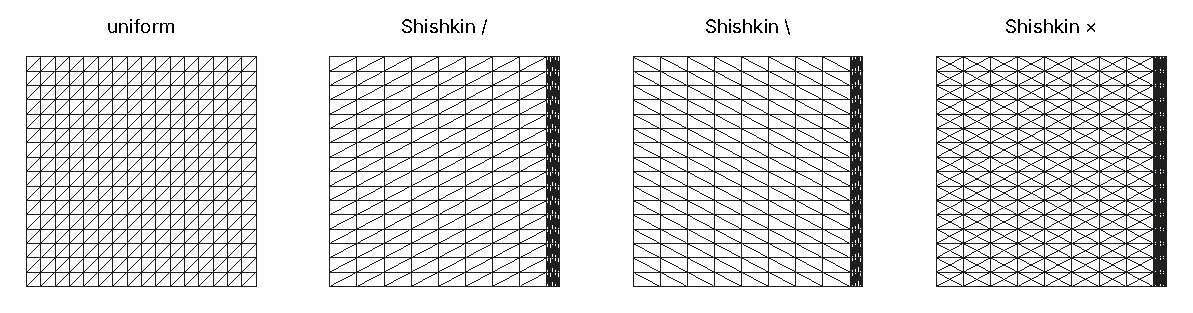
\includegraphics[width=\textwidth]{aniso_meshes.pdf}
\caption{Uniform and Shishkin meshes with the splittings ``/'', ``\textbackslash'' and crossed for the problem with
parabolic layers, $n=16$, drawn for $\eps=10^{-2}$ so that the layer regions are visible.}\label{fig:meshes}
\end{figure}

% generated by galerkit examples/convection_diffusion/2d/anisotropic_afc/make_report.py; do not edit
\begin{table}[!htbp]
\centering\scriptsize\setlength{\tabcolsep}{3pt}
\caption{The meshes at $n=128$: nodes, largest aspect ratio (longest edge over its height), shortest edge, largest angle, and the edges with a positive off-diagonal entry of the $P_1$ Laplace matrix (not Delaunay).}\label{tab:mesh}
\begin{tabular}{llrrrrr}
\toprule
case & mesh & nodes & aspect & $h_{\min}$ & max angle & Laplace $>0$\\
\midrule
\texttt{exp\_layer}, $\varepsilon=10^{-4}$ & uniform & 16641 & $2.0\mathrm{e}{0}$ & $7.8\mathrm{e}{-3}$ & 90.0 & 0 \\
\texttt{exp\_layer}, $\varepsilon=10^{-4}$ & Shishkin / & 16641 & $5.2\mathrm{e}{2}$ & $1.5\mathrm{e}{-5}$ & 90.0 & 0 \\
\texttt{exp\_layer}, $\varepsilon=10^{-4}$ & Shishkin \textbackslash & 16641 & $5.2\mathrm{e}{2}$ & $1.5\mathrm{e}{-5}$ & 90.0 & 0 \\
\texttt{exp\_layer}, $\varepsilon=10^{-4}$ & Shishkin $\times$ & 33025 & $1.0\mathrm{e}{3}$ & $1.5\mathrm{e}{-5}$ & 179.8 & 16320 \\
\texttt{exp\_layer}, $\varepsilon=10^{-8}$ & uniform & 16641 & $2.0\mathrm{e}{0}$ & $7.8\mathrm{e}{-3}$ & 90.0 & 0 \\
\texttt{exp\_layer}, $\varepsilon=10^{-8}$ & Shishkin / & 16641 & $5.2\mathrm{e}{6}$ & $1.5\mathrm{e}{-9}$ & 90.0 & 0 \\
\texttt{exp\_layer}, $\varepsilon=10^{-8}$ & Shishkin \textbackslash & 16641 & $5.2\mathrm{e}{6}$ & $1.5\mathrm{e}{-9}$ & 90.0 & 0 \\
\texttt{exp\_layer}, $\varepsilon=10^{-8}$ & Shishkin $\times$ & 33025 & $1.0\mathrm{e}{7}$ & $1.5\mathrm{e}{-9}$ & 180.0 & 16320 \\
\texttt{boundary\_layers}, $\varepsilon=10^{-8}$ & uniform & 16641 & $2.0\mathrm{e}{0}$ & $7.8\mathrm{e}{-3}$ & 90.0 & 0 \\
\texttt{boundary\_layers}, $\varepsilon=10^{-8}$ & Shishkin / & 16641 & $3.1\mathrm{e}{7}$ & $5.1\mathrm{e}{-10}$ & 90.0 & 0 \\
\texttt{boundary\_layers}, $\varepsilon=10^{-8}$ & Shishkin \textbackslash & 16641 & $3.1\mathrm{e}{7}$ & $5.1\mathrm{e}{-10}$ & 90.0 & 0 \\
\texttt{boundary\_layers}, $\varepsilon=10^{-8}$ & Shishkin $\times$ & 33025 & $6.2\mathrm{e}{7}$ & $4.6\mathrm{e}{-10}$ & 180.0 & 12224 \\
\texttt{parabolic\_layers}, $\varepsilon=10^{-8}$ & uniform & 16641 & $2.0\mathrm{e}{0}$ & $7.8\mathrm{e}{-3}$ & 90.0 & 0 \\
\texttt{parabolic\_layers}, $\varepsilon=10^{-8}$ & Shishkin / & 16641 & $1.0\mathrm{e}{7}$ & $1.5\mathrm{e}{-9}$ & 90.0 & 0 \\
\texttt{parabolic\_layers}, $\varepsilon=10^{-8}$ & Shishkin \textbackslash & 16641 & $1.0\mathrm{e}{7}$ & $1.5\mathrm{e}{-9}$ & 90.0 & 0 \\
\texttt{parabolic\_layers}, $\varepsilon=10^{-8}$ & Shishkin $\times$ & 33025 & $2.1\mathrm{e}{7}$ & $1.5\mathrm{e}{-9}$ & 180.0 & 16320 \\
\bottomrule
\end{tabular}
\end{table}


\subsection{Layers along circular arcs}\label{sec:polar}

For the convection field $\bb=(-y,x)$ the characteristics are circles around the origin, and layers created at the
inflow boundary $y=0$ follow arcs $r=\sqrt{x^2+y^2}=\text{const}$. A tensor-product mesh can be aligned with such
layers only near the inflow and the outflow boundary. We therefore use a polar mesh of the unit square: rings
$r=r_k$, $0=r_0<\dots<r_K=0.9$, a few further rings that blend the circle $r=0.9$ into the boundary of the square,
and $n$ uniform angular intervals in $[0,\pi/2]$; the cells around the origin form a fan, all other quadrilaterals are
split into two triangles. The radii are uniform (\emph{polar mesh}), or refined in the spirit of Shishkin meshes
around the arcs carrying the layers (\emph{layer-adapted polar mesh}). In the latter, the cells in the layer regions
are long in the angular direction and short in the radial one.

%=====================================================================================================
\section{Modifications of the stabilization on anisotropic meshes}\label{sec:switch}
%=====================================================================================================

On a layer-adapted mesh, the Galerkin method is stable in the layer regions, and the artificial diffusion of the
algebraic stabilizations might be needed only where the mesh does not resolve the solution. A first idea is to switch
the stabilization off, i.e., to set $d_{ij}=b_{ij}=0$, on all edges with mesh P\'eclet number
\begin{equation}\label{eq:pe}
  \mathrm{Pe}_E=\frac{|\bb(x_E)|\,|E|}{2\eps}\le1,
\end{equation}
where $x_E$ is the midpoint of $E$. We use the full speed $|\bb|$ instead of the component of $\bb$ along $E$, since
otherwise the crosswind edges of coarse cells would be regarded as resolved.

The second, and as it turns out the effective, modification switches the stabilization off on the edges along the
layers: $d_{ij}=b_{ij}=0$ on every edge $E$ such that all cells $K$ containing $E$ have an aspect ratio
$\mathrm{diam}(K)^2/(2|K|)\ge\kappa$ and $|E|\ge\frac12\mathrm{diam}(K)$, i.e., $E$ is a long edge of every adjacent
cell. We use $\kappa=10$ on the tensor-product meshes and $\kappa=3$ on the polar meshes, whose layer cells are only
moderately stretched. The criterion uses only the mesh. On a layer-adapted mesh, the long edges of the layer cells are
directed along the layer, where the solution varies slowly, and the edges across the layer remain stabilized.

\begin{remark}
On the switched-off edges the scheme is the Galerkin method, and the sufficient conditions for the DMP are lost on
those of them with $\max\{a_{ij},a_{ji}\}>0$. In our computations these edges are counted. On meshes of right
triangles they arise only from the reaction term.
\end{remark}

Finally, the limiters of the BJK, Kuzmin, MUAS and SMUAS methods are built from the quantities
$R_i=\min\{1,Q_i/P_i\}$, with local bounds $Q_i$ and sums of antidiffusive fluxes $P_i$. A relaxed version $R_i=\min\{1,\mu Q_i/P_i\}$, $\mu>1$, as in
\cite[(27)]{Kno23} for the Kuzmin limiter, limits less and clips smooth extrema less; the DMP is then no longer
guaranteed. We use $\mu=2$ in the last example.

%=====================================================================================================
\section{Nonlinear solvers}\label{sec:solvers}
%=====================================================================================================

The standard solver for \eqref{eq:as} is the fixed point iteration with the right-hand side updated
\cite{BJK16,JJ19}: with the matrix $D=(d_{ij})$, which is independent of $u$, solve
\begin{equation}\label{eq:fprhs}
  (A+D)\tilde u=g-\bigl(B(u^k)-D\bigr)u^k,\qquad u^{k+1}=u^k+\omega_k(\tilde u-u^k),
\end{equation}
where $\omega_k$ is adapted to the decrease of the residual. Only one matrix factorization is needed. We stop
when the Euclidean norm of the residual is below $10^{-10}$, or after 3000 iterations.

The Anderson acceleration of \eqref{eq:fprhs} with depth 10 \cite{WN11}, without damping, diverges for F-BBK and S-BBK,
for which the undamped fixed point map is expansive. We therefore use a non-monotone safeguard: an accelerated iterate
is accepted only if its residual is smaller than the largest of the last ten residuals; otherwise, a damped fixed
point step is taken and the history is cleared. A monotone safeguard rejected about every second step and destroyed
the acceleration.

Newton's method for \eqref{eq:as} is a semismooth Newton method, since the limiters are built from $\max$, $\min$,
$|\cdot|$, $\min\{1,Q/P\}$, local extrema, and choices according to the sign of fluxes. In the spirit of the
differentiable shock detectors of \cite{BB17}, we replace each of these building blocks by a $C^1$ function with an
error of order $\sigma$, e.g., $x^+\mapsto(x^+)^2/(x^++\sigma)$, and the local extrema by a log-sum-exp. The
regularized $b_{ij}(u)$ converge to the original ones with $O(\sigma)$ for all methods except MC, which we did not
regularize. The Jacobian of the regularized scheme is computed exactly by a sparse forward differentiation of the same
code that evaluates $b_{ij}(u)$. Newton's method with line search is applied for
$\sigma=10^{-1},10^{-2},\dots,10^{-6}$, each stage starting from the previous solution, followed by at most 20 Newton
steps for the original scheme. A problem counts as solved only if this last stage reaches the residual $10^{-10}$ for
the original scheme.

%=====================================================================================================
\section{Numerical studies}\label{sec:num}
%=====================================================================================================

This section presents the numerical results. All computations were performed with the Python finite element package
galerkit; the scripts and the data of all runs are available in its branch \texttt{feature/anisotropic-afc}.
% TODO: repository link / Zenodo DOI.
We consider $n=16,32,64,128$, i.e., meshes with up to 16\,641 nodes (33\,153 with the crossed splitting). The
Galerkin and SUPG methods serve as references.

\subsection{Examples and error measures}

All examples are posed in $\Omega=(0,1)^2$. The problem names in the tables are those of galerkit.

\paragraph{Example 1 (exponential layer, \texttt{exp\_layer}).} $\bb=(1,0)$, $c=f=0$, and the solution
$u(x,y)=(1-e^{(x-1)/\eps})/(1-e^{-1/\eps})\in[0,1]$, with an exponential layer at $x=1$, for $\eps=10^{-4},10^{-8}$.
Since $f=c=0$, the local DMP holds and its violations can be counted node by node.

\paragraph{Example 2 (boundary layers, \texttt{boundary\_layers}).} $\eps=10^{-8}$, $\bb=(2,3)$, $c=1$, and $f$ and $u_b$
chosen such that the solution has exponential layers at $x=1$ and $y=1$.
% TODO: state the solution formula as in galerkit (u = xy^2 - y^2 e^{2(x-1)/eps} - x e^{3(y-1)/eps} + e^{(2(x-1)+3(y-1))/eps}).

\paragraph{Example 3 (parabolic layers, \texttt{parabolic\_layers}).} $\eps=10^{-8}$, $\bb=(1,0)$, $c=0$, $f=1$,
$u_b=0$ \cite{JK07}: an exponential layer at $x=1$ and parabolic layers at $y=0$ and $y=1$. The solution is not
known, but $0\le u\le x\le1$.

\paragraph{Example 4 (straight interior layer, \texttt{interior\_layer}).} $\eps=10^{-8}$, $\bb=(1,0)$, $c=f=0$, $u_b=1$
on $\{x=0,\ y>\frac12\}$ and on $\{y=1,\ x<1\}$, and $u_b=0$ elsewhere, also at the outflow boundary $x=1$. The jump of
the inflow data creates an interior parabolic layer along $y=\frac12$ of width $O(\sqrt{\eps x})$, and there is an
exponential outflow layer at $x=1$ for $y>\frac12$. Away from the outflow layer, the function
\begin{equation*}
  u_{\rm ref}(x,y)=\tfrac12\,\mathrm{erfc}\Bigl(\frac{1/2-y}{2\sqrt{\eps x}}\Bigr)
\end{equation*}
solves $u_x=\eps u_{yy}$ exactly; the neglected term $\eps u_{xx}$ is negligible for $\eps=10^{-8}$, and we use
$u_{\rm ref}$ as reference solution.

\paragraph{Example 5 (layers along circular arcs, \texttt{rotating\_profile}).} The steady problem of
\cite[Sect.~7]{arXiv2204}: $\eps=10^{-5}$, $\bb=(-y,x)$, $c=f=0$, the inflow profile
\begin{equation*}
  u(x,0)=\begin{cases}\frac{x-0.375}{\xi}+1, & x\in[0.375-\xi,0.375),\\
  -0.75\,\frac{x-0.5}{0.125}+0.25, & x\in[0.375,0.5),\\
  0.25\,\frac{x-0.625}{0.125}+0.5, & x\in[0.5,0.625),\\
  -0.5\,\frac{x-0.625}{\xi}+0.5, & x\in[0.625,0.625+\xi),\\
  32(x-0.75)(1-x), & x\in[0.75,1],\\ 0 & \text{else},\end{cases}\qquad\xi=10^{-3},
\end{equation*}
$u=0$ at $x=1$, and homogeneous Neumann conditions at the outflow boundaries $x=0$ and $y=1$. The profile is
transported along circles: steep interior layers along the arcs $r\approx0.375$ and $r\approx0.625$, weak layers along
$r=0.5$ and $r=0.75$ where the profile has kinks, and a smooth hump; $0\le u\le1$. In polar coordinates,
$\bb\cdot\nabla u=u_\theta$, and neglecting $\eps u_{\theta\theta}/r^2$, which is small compared with $\eps u_{rr}$ in
the thin layers, the problem becomes the radial heat equation $u_\theta=\eps(u_{rr}+u_r/r)$ in the ``time''
$\theta\in[0,\pi/2]$ with the inflow profile as initial condition. We solve this equation with $4\cdot10^4$ radial
cells and 4000 Crank--Nicolson steps; halving both changes the solution by $3\cdot10^{-5}$. This solution serves as
reference.

\paragraph{Error measures.} We report the error in $L^2(\Omega)$, the maximal nodal error, and the maximal nodal
error away from the layer regions. The energy norm is not used since on uniform meshes the quadrature does not see
layers of width $\eps$. For Examples~4 and~5 the errors are computed against the reference solutions in the regions
where these are valid: in Example~4 for $x\le1-\tau_x$ (the $L^2$ error) and for $0.1\le x\le1-\tau_x$ (the maximal
nodal error), since no mesh resolves the layer width $\sqrt{\eps x}\to0$ at the inflow corner; in Example~5 for $r\le1$.
For the DMP, we check the mesh conditions of Table~\ref{tab:methods}, the local DMP in Example~1, and the bounds of the
exact solution in Examples~3--5. Results of runs whose nonlinear problem was not solved are those of the best iterate
and are marked in the tables.

\subsection{Accuracy on Shishkin meshes}

Figure~\ref{fig:errors} and Tables~\ref{tab:acc-exp_layer-1e-08}--\ref{tab:acc-boundary_layers-1e-08} present the
errors on the uniform meshes and on the Shishkin meshes with the splittings ``/'' and crossed.

\begin{figure}[!htbp]\centering
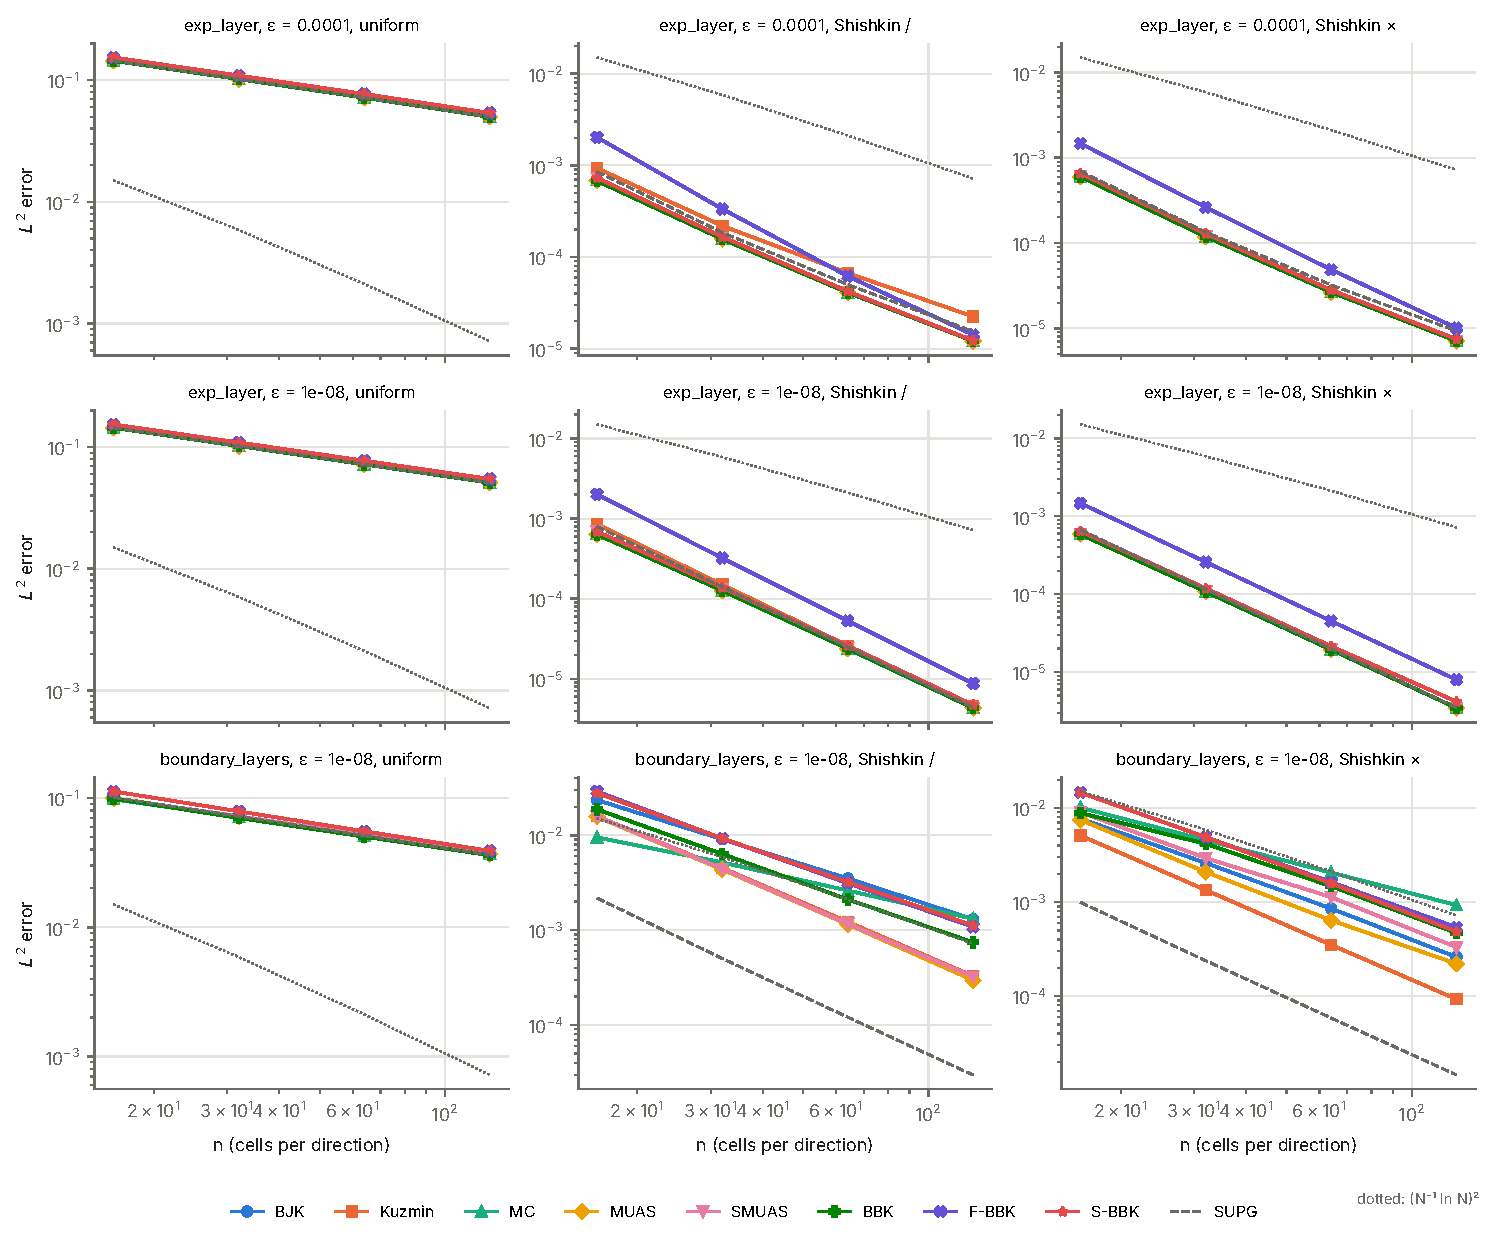
\includegraphics[width=\textwidth]{aniso_errors.pdf}
\caption{Examples 1--3: $L^2$ errors on uniform, Shishkin ``/'' and crossed Shishkin meshes.}\label{fig:errors}
\end{figure}

% generated by galerkit examples/convection_diffusion/2d/anisotropic_afc/make_report.py; do not edit
\begin{table}[!htbp]
\centering\scriptsize\setlength{\tabcolsep}{3pt}
\caption{\texttt{exp\_layer}, $\varepsilon=10^{-4}$, $n=128$: maximal nodal error, its order in $n$ (between $n=64$ and 128), and the $L^2$ error.}\label{tab:acc-exp_layer-1e-04}
\begin{tabular}{l rrr rrr rrr}
\toprule
 & \multicolumn{3}{c}{uniform} & \multicolumn{3}{c}{Shishkin /} & \multicolumn{3}{c}{Shishkin $\times$}\\
method & max & ord. & $L^2$ & max & ord. & $L^2$ & max & ord. & $L^2$\\
\midrule
Galerkin & $1.6\mathrm{e}{0}$ & 0.51 & $1.6\mathrm{e}{-1}$ & $7.8\mathrm{e}{-4}$ & 1.61 & $2.3\mathrm{e}{-5}$ & $9.4\mathrm{e}{-4}$ & 1.53 & $8.1\mathrm{e}{-6}$ \\
SUPG & $2.3\mathrm{e}{-14}$ & -1.86 & $5.0\mathrm{e}{-2}$ & $1.6\mathrm{e}{-13}$ & -2.56 & $1.5\mathrm{e}{-5}$ & $8.7\mathrm{e}{-4}$ & 1.45 & $9.3\mathrm{e}{-6}$ \\
BJK & $1.6\mathrm{e}{-14}$ & -1.04 & $5.0\mathrm{e}{-2}$ & $7.7\mathrm{e}{-4}$ & 1.56 & $1.2\mathrm{e}{-5}$ & $9.4\mathrm{e}{-4}$ & 1.53 & $7.1\mathrm{e}{-6}$ \\
Kuzmin & $1.5\mathrm{e}{-14}$ & -1.01 & $5.0\mathrm{e}{-2}$ & $3.0\mathrm{e}{-3}$ & 0.95 & $2.2\mathrm{e}{-5}$ & $9.4\mathrm{e}{-4}$ & 1.53 & $7.1\mathrm{e}{-6}$ \\
MC & $1.5\mathrm{e}{-14}$ & -1.01 & $5.0\mathrm{e}{-2}$ & $7.8\mathrm{e}{-4}$ & 1.57 & $1.2\mathrm{e}{-5}$ & $9.4\mathrm{e}{-4}$ & 1.53 & $7.1\mathrm{e}{-6}$ \\
MUAS & $1.5\mathrm{e}{-14}$ & -1.01 & $5.0\mathrm{e}{-2}$ & $7.7\mathrm{e}{-4}$ & 1.56 & $1.2\mathrm{e}{-5}$ & $9.4\mathrm{e}{-4}$ & 1.53 & $7.1\mathrm{e}{-6}$ \\
SMUAS & $1.5\mathrm{e}{-14}$ & -1.01 & $5.0\mathrm{e}{-2}$ & $7.7\mathrm{e}{-4}$ & 1.56 & $1.2\mathrm{e}{-5}$ & $9.4\mathrm{e}{-4}$ & 1.53 & $7.1\mathrm{e}{-6}$ \\
BBK & $1.5\mathrm{e}{-14}$ & -1.01 & $5.0\mathrm{e}{-2}$ & $7.7\mathrm{e}{-4}$ & 1.56 & $1.2\mathrm{e}{-5}$ & $9.4\mathrm{e}{-4}$ & 1.53 & $7.1\mathrm{e}{-6}$ \\
F-BBK & $1.2\mathrm{e}{-1}$ & -0.01 & $5.4\mathrm{e}{-2}$ & $7.9\mathrm{e}{-4}$ & 1.51 & $1.4\mathrm{e}{-5}$ & $9.4\mathrm{e}{-4}$ & 1.53 & $1.0\mathrm{e}{-5}$ \\
S-BBK & $1.2\mathrm{e}{-1}$ & -0.01 & $5.4\mathrm{e}{-2}$ & $7.8\mathrm{e}{-4}$ & 1.55 & $1.2\mathrm{e}{-5}$ & $9.4\mathrm{e}{-4}$ & 1.53 & $7.4\mathrm{e}{-6}$ \\
\bottomrule
\end{tabular}
\end{table}

\begin{table}[!htbp]
\centering\scriptsize\setlength{\tabcolsep}{3pt}
\caption{\texttt{exp\_layer}, $\varepsilon=10^{-8}$, $n=128$: maximal nodal error, its order in $n$ (between $n=64$ and 128), and the $L^2$ error.}\label{tab:acc-exp_layer-1e-08}
\begin{tabular}{l rrr rrr rrr}
\toprule
 & \multicolumn{3}{c}{uniform} & \multicolumn{3}{c}{Shishkin /} & \multicolumn{3}{c}{Shishkin $\times$}\\
method & max & ord. & $L^2$ & max & ord. & $L^2$ & max & ord. & $L^2$\\
\midrule
Galerkin & $2.4\mathrm{e}{3}$ & 1.44 & $6.1\mathrm{e}{2}$ & $8.4\mathrm{e}{-4}$ & 1.59 & $7.2\mathrm{e}{-5}$ & $7.2\mathrm{e}{-3}$ & 1.15 & $4.7\mathrm{e}{-4}$ \\
SUPG & $2.8\mathrm{e}{-14}$ & -1.32 & $5.1\mathrm{e}{-2}$ & $7.2\mathrm{e}{-14}$ & -1.65 & $4.4\mathrm{e}{-6}$ & $8.7\mathrm{e}{-4}$ & 1.45 & $3.5\mathrm{e}{-6}$ \\
BJK & $1.5\mathrm{e}{-14}$ & -1.40 & $5.1\mathrm{e}{-2}$ & $7.7\mathrm{e}{-4}$ & 1.56 & $4.3\mathrm{e}{-6}$ & $9.4\mathrm{e}{-4}$ & 1.53 & $3.5\mathrm{e}{-6}$ \\
Kuzmin & $1.5\mathrm{e}{-14}$ & -1.40 & $5.1\mathrm{e}{-2}$ & $3.0\mathrm{e}{-3}$ & 0.95 & $4.5\mathrm{e}{-6}$ & $9.4\mathrm{e}{-4}$ & 1.53 & $3.5\mathrm{e}{-6}$ \\
MC & $1.5\mathrm{e}{-14}$ & -1.40 & $5.1\mathrm{e}{-2}$ & $7.8\mathrm{e}{-4}$ & 1.57 & $4.3\mathrm{e}{-6}$ & $9.4\mathrm{e}{-4}$ & 1.53 & $3.5\mathrm{e}{-6}$ \\
MUAS & $1.5\mathrm{e}{-14}$ & -1.40 & $5.1\mathrm{e}{-2}$ & $7.7\mathrm{e}{-4}$ & 1.56 & $4.3\mathrm{e}{-6}$ & $9.4\mathrm{e}{-4}$ & 1.53 & $3.5\mathrm{e}{-6}$ \\
SMUAS & $1.5\mathrm{e}{-14}$ & -1.40 & $5.1\mathrm{e}{-2}$ & $7.7\mathrm{e}{-4}$ & 1.56 & $4.3\mathrm{e}{-6}$ & $9.4\mathrm{e}{-4}$ & 1.53 & $3.5\mathrm{e}{-6}$ \\
BBK & $1.5\mathrm{e}{-14}$ & -1.40 & $5.1\mathrm{e}{-2}$ & $7.7\mathrm{e}{-4}$ & 1.56 & $4.3\mathrm{e}{-6}$ & $9.4\mathrm{e}{-4}$ & 1.53 & $3.5\mathrm{e}{-6}$ \\
F-BBK & $1.2\mathrm{e}{-1}$ & -0.00 & $5.5\mathrm{e}{-2}$ & $7.9\mathrm{e}{-4}$ & 1.51 & $8.7\mathrm{e}{-6}$ & $9.4\mathrm{e}{-4}$ & 1.53 & $8.0\mathrm{e}{-6}$ \\
S-BBK & $1.2\mathrm{e}{-1}$ & -0.00 & $5.5\mathrm{e}{-2}$ & $7.8\mathrm{e}{-4}$ & 1.55 & $4.7\mathrm{e}{-6}$ & $9.4\mathrm{e}{-4}$ & 1.53 & $4.2\mathrm{e}{-6}$ \\
\bottomrule
\end{tabular}
\end{table}

\begin{table}[!htbp]
\centering\scriptsize\setlength{\tabcolsep}{3pt}
\caption{\texttt{boundary\_layers}, $\varepsilon=10^{-8}$, $n=128$: maximal nodal error, its order in $n$ (between $n=64$ and 128), and the $L^2$ error.}\label{tab:acc-boundary_layers-1e-08}
\begin{tabular}{l rrr rrr rrr}
\toprule
 & \multicolumn{3}{c}{uniform} & \multicolumn{3}{c}{Shishkin /} & \multicolumn{3}{c}{Shishkin $\times$}\\
method & max & ord. & $L^2$ & max & ord. & $L^2$ & max & ord. & $L^2$\\
\midrule
Galerkin & $7.0\mathrm{e}{0}$ & 0.06 & $1.6\mathrm{e}{0}$ & $1.5\mathrm{e}{-2}$ & 0.78 & $6.5\mathrm{e}{-5}$ & $1.9\mathrm{e}{-3}$ & 1.34 & $3.3\mathrm{e}{-5}$ \\
SUPG & $2.9\mathrm{e}{-1}$ & -0.04 & $3.6\mathrm{e}{-2}$ & $1.7\mathrm{e}{-2}$ & 0.89 & $3.0\mathrm{e}{-5}$ & $3.2\mathrm{e}{-3}$ & 1.30 & $1.5\mathrm{e}{-5}$ \\
BJK & $5.3\mathrm{e}{-2}$ & 0.82 & $3.6\mathrm{e}{-2}$ & $2.1\mathrm{e}{-2}$ & 0.96 & $1.3\mathrm{e}{-3}$ & $1.3\mathrm{e}{-2}$ & 0.90 & $2.6\mathrm{e}{-4}$ \\
Kuzmin & $1.6\mathrm{e}{-2}$ & 0.98 & $3.7\mathrm{e}{-2}$ & $4.5\mathrm{e}{-2}$ & 0.64 & $3.3\mathrm{e}{-4}$ & $3.1\mathrm{e}{-2}$ & 0.61 & $9.3\mathrm{e}{-5}$ \\
MC & $2.5\mathrm{e}{-2}$ & 0.94 & $3.7\mathrm{e}{-2}$ & $4.0\mathrm{e}{-2}$ & 0.59 & $1.3\mathrm{e}{-3}$ & $5.9\mathrm{e}{-2}$ & 0.56 & $9.3\mathrm{e}{-4}$ \\
MUAS & $1.6\mathrm{e}{-2}$ & 0.98 & $3.7\mathrm{e}{-2}$ & $2.4\mathrm{e}{-2}$ & 0.72 & $3.0\mathrm{e}{-4}$ & $6.5\mathrm{e}{-2}$ & 0.57 & $2.2\mathrm{e}{-4}$ \\
SMUAS & $1.6\mathrm{e}{-2}$ & 0.97 & $3.7\mathrm{e}{-2}$ & $3.2\mathrm{e}{-2}$ & 0.19 & $3.2\mathrm{e}{-4}$ & $2.9\mathrm{e}{-2}$ & 1.43 & $3.3\mathrm{e}{-4}$ \\
BBK & $6.8\mathrm{e}{-2}$ & 0.74 & $3.6\mathrm{e}{-2}$ & $3.0\mathrm{e}{-2}$ & 0.67 & $7.4\mathrm{e}{-4}$ & $3.2\mathrm{e}{-2}$ & 0.56 & $4.7\mathrm{e}{-4}$ \\
F-BBK & $1.7\mathrm{e}{-1}$ & 0.21 & $3.9\mathrm{e}{-2}$ & $2.9\mathrm{e}{-2}$ & 0.97 & $1.1\mathrm{e}{-3}$ & $1.8\mathrm{e}{-2}$ & 0.97 & $5.4\mathrm{e}{-4}$ \\
S-BBK & $1.7\mathrm{e}{-1}$ & 0.21 & $3.9\mathrm{e}{-2}$ & $3.7\mathrm{e}{-2}$ & 0.69 & $1.1\mathrm{e}{-3}$ & $2.9\mathrm{e}{-2}$ & 0.69 & $4.9\mathrm{e}{-4}$ \\
\bottomrule
\end{tabular}
\end{table}


The Shishkin meshes resolve the layers. For Example~1 with $\eps=10^{-8}$, the $L^2$ error at $n=128$ drops from
$5\cdot10^{-2}$ on the uniform mesh to about $4\cdot10^{-6}$ for every method, with almost the rate
$(n^{-1}\ln n)^2$ and independently of $\eps$. On the uniform mesh, the nodal values of this layer, which is aligned
with the mesh, are exact for most methods although the layer is not resolved, so that the maximal nodal error alone is
not a measure of quality here.

The algebraic stabilizations pay a price on the layer-adapted meshes. In Example~2 on the ``/'' Shishkin mesh, the
Galerkin method ($L^2$ error $6.5\cdot10^{-5}$ at $n=128$) and the SUPG method ($3\cdot10^{-5}$) converge with order 2,
whereas the algebraic methods are 5 to 40 times less accurate: Kuzmin and MUAS $3\cdot10^{-4}$ with an order of about
1.9, BJK and BBK $0.7$--$1.3\cdot10^{-3}$ with order 1.5, and MC $1.3\cdot10^{-3}$ with order 1. Away from the layers,
their maximal errors of about $10^{-2}$ converge only with order 0.7--1, against 1.6--1.8 for the Galerkin and SUPG
methods. On a mesh that resolves the layers, the Galerkin method is stable, and the artificial diffusion of the
limiters only adds a first-order consistency error. The splittings ``/'' and ``\textbackslash'' give almost the same
errors. The crossed splitting doubles the number of nodes and gives the same accuracy for Example~1, but changes the
ordering of the methods in Example~2, with Kuzmin and MUAS being the most accurate.

The large error of the algebraic methods in Example~2 is located at the transition corner $(1-\tau_x,1-\tau_y)$: at
$n=64$, their maximal error away from the layers is $2.3\cdot10^{-2}$, while in the interior of the coarse region they
are as accurate as the Galerkin method ($1.9\cdot10^{-3}$ against $1.5\cdot10^{-3}$). This error originates from the
long edges inside the layer strips. These edges have length $1/n$ along the layer, $\bb=(2,3)$ has a component along
them, hence $\mathrm{Pe}_E\gg1$, and the limiters add diffusion along the layer. Consequently, switching the
stabilization off according to the P\'eclet criterion \eqref{eq:pe} does not help: it regards exactly these edges as
unresolved. The artificial diffusion $d_{ij}$ already vanishes on the diffusion-dominated edges of right triangles,
and in Examples~1 and~3 none of the 8\,128--32\,640 edges with $\mathrm{Pe}_E\le1$ at $n=128$ has $d_{ij}\neq0$. In
Example~2 the criterion acts on about 4\,000 edges where the non-lumped reaction term makes $\max\{a_{ij},a_{ji}\}>0$,
but the errors and iteration numbers change by a few per cent only.

\subsection{The discrete maximum principle}

% generated by galerkit examples/convection_diffusion/2d/anisotropic_afc/make_report.py; do not edit
\begin{table}[!htbp]
\centering\scriptsize\setlength{\tabcolsep}{2.5pt}
\caption{DMP at $n=128$: ``ok'' if the sufficient mesh condition of the method holds on every edge, otherwise the number of edges where it fails (\mism{colour}); for \texttt{exp\_layer} ($f=c=0$) a second number gives the nodes violating the local DMP; $^\dagger$: the solution leaves the bounds of the exact solution by more than $10^{-8}$.}\label{tab:dmp}
\resizebox{\textwidth}{!}{\begin{tabular}{l rrr rrr rrr rrr}
\toprule
 & \multicolumn{3}{c}{\texttt{exp\_layer}, $\varepsilon=10^{-4}$} & \multicolumn{3}{c}{\texttt{exp\_layer}, $\varepsilon=10^{-8}$} & \multicolumn{3}{c}{\texttt{boundary\_layers}, $\varepsilon=10^{-8}$} & \multicolumn{3}{c}{\texttt{parabolic\_layers}, $\varepsilon=10^{-8}$}\\
method & u & / & $\times$ & u & / & $\times$ & u & / & $\times$ & u & / & $\times$\\
\midrule
BJK & ok & ok & ok & ok & ok & ok & ok & ok & ok & ok$^\dagger$ & ok$^\dagger$ & ok$^\dagger$ \\
Kuzmin & ok & ok & \mism{8192} & ok & ok & \mism{8192} & ok & ok & \mism{12224} & ok & ok$^\dagger$ & \mism{8192} \\
MC & ok & ok & \mism{8192} & ok & ok & \mism{8192} & ok & ok & \mism{12224} & ok & ok & \mism{8192} \\
MUAS & ok & ok & ok & ok & ok & ok & ok & ok & ok & ok & ok$^\dagger$ & ok \\
SMUAS & ok & ok & ok & ok & ok & ok & ok & ok & ok & ok & ok & ok \\
BBK & ok & ok & ok & ok & ok & ok & ok & ok & ok & ok & ok$^\dagger$ & ok \\
F-BBK & ok & ok & \mism{8064} & ok & ok & \mism{8064} & ok & ok & \mism{12224} & ok & ok$^\dagger$ & -- \\
S-BBK & ok & ok & \mism{8064} & ok & ok & \mism{8064} & ok & ok & \mism{12224} & ok & ok$^\dagger$ & -- \\
\bottomrule
\end{tabular}}
\end{table}


Table~\ref{tab:dmp} shows that the conditions of Table~\ref{tab:methods} are satisfied on every edge of the uniform
meshes and of the Shishkin meshes with two triangles per rectangle, for all problems. In Example~2, the non-lumped
reaction term ($c=1$) does not violate $\min\{a_{ij},a_{ji}\}\le0$ since convection dominates. On the crossed
Shishkin meshes, the obtuse angles make diffusion entries positive, and the Kuzmin and MC condition is violated on 128
to 12\,224 edges, the condition of F-BBK and S-BBK at the larger $n$ (8\,064 edges for Example~1 at $n=128$).

We stress the fact that no violation of the DMP is observed nevertheless. In Example~1, where the local DMP applies, no
method violates it on any mesh, including the Kuzmin and MC methods on the crossed meshes. In Example~3, no method
undershoots the bound $u\ge0$. On the ``/'' and ``\textbackslash'' Shishkin meshes of Example~3, however, the BJK,
Kuzmin, MUAS, BBK, F-BBK and S-BBK methods exceed the bound $u\le1$ of the exact solution by up to 9\,\%. This is not a
violation of the DMP, since $f=1$, but it is non-physical. The MC and SMUAS methods stay below $1+6\cdot10^{-4}$, and
no method overshoots on the crossed meshes.

\subsection{Nonlinear iterations and the type of the layer-adapted mesh}

\begin{figure}[!htbp]\centering
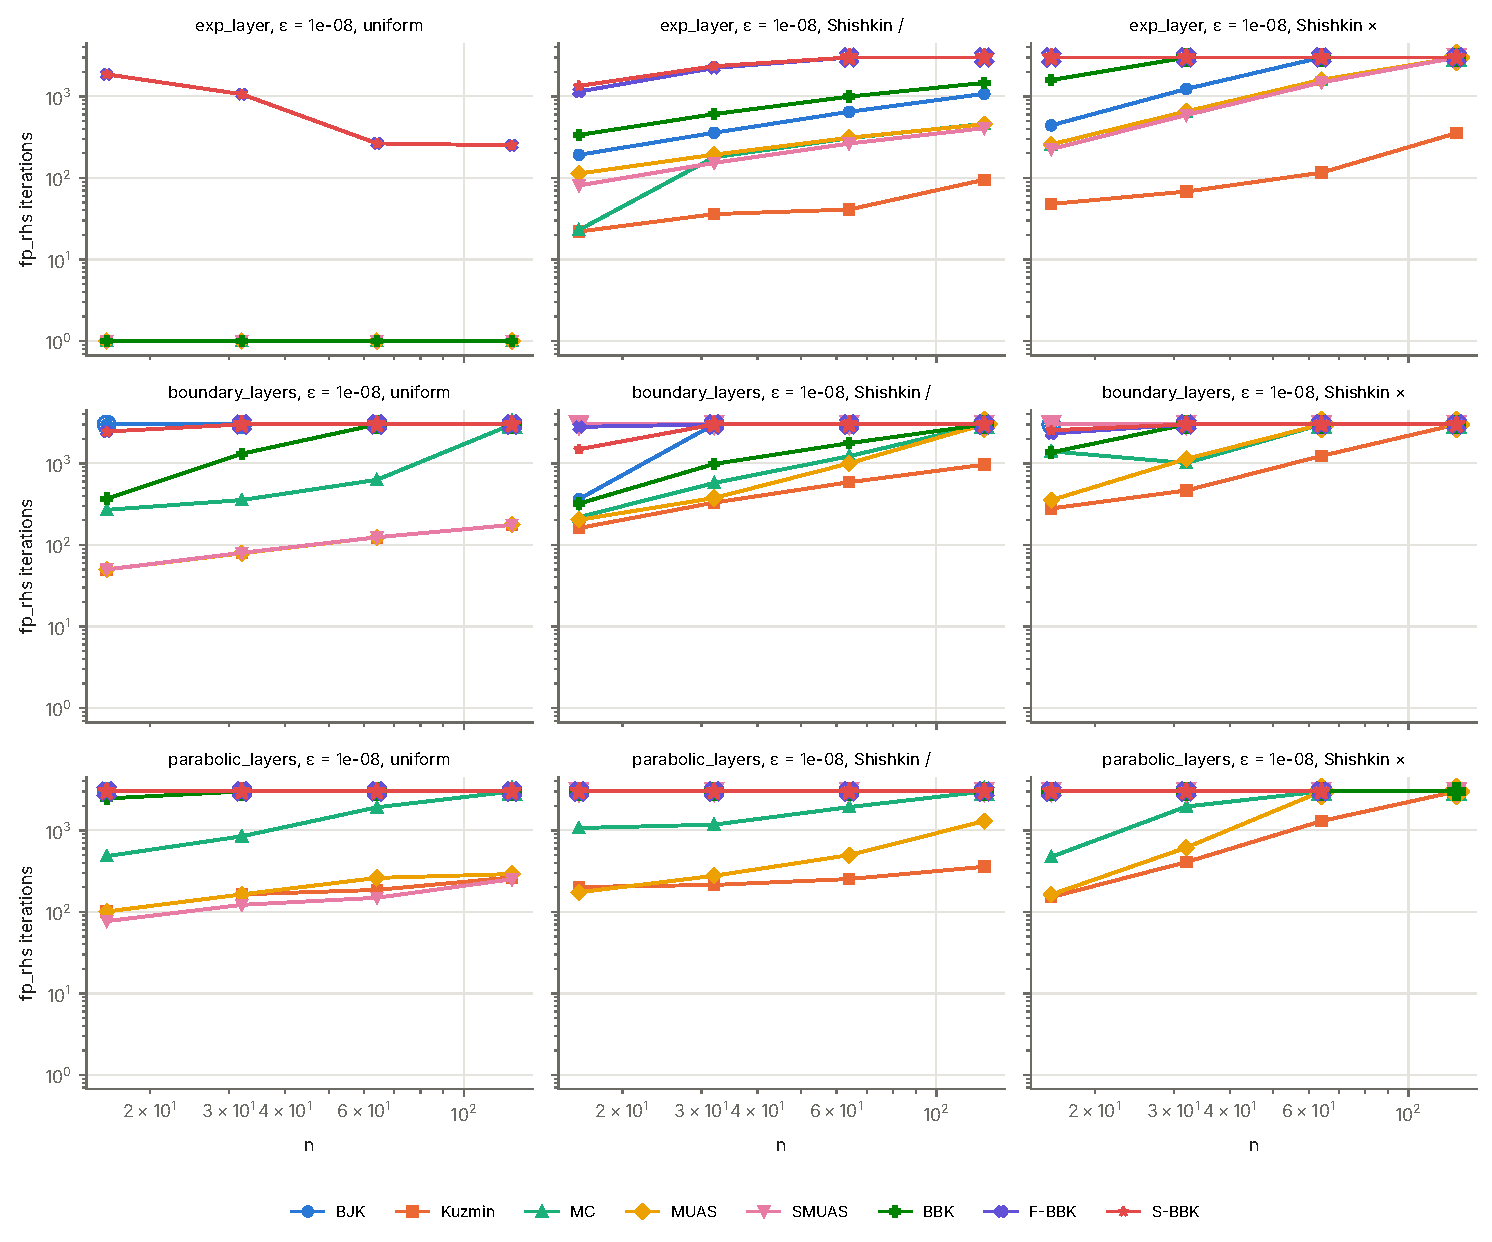
\includegraphics[width=\textwidth]{aniso_iterations.pdf}
\caption{Examples 1--3: iterations of the fixed point method \eqref{eq:fprhs}; open symbols: not converged within 3000
iterations.}\label{fig:it}
\end{figure}

% generated by galerkit examples/convection_diffusion/2d/anisotropic_afc/make_report.py; do not edit
\begin{table}[!htbp]
\centering\scriptsize\setlength{\tabcolsep}{2.5pt}
\caption{Iterations of the fixed point rhs at $n=128$ (u: uniform, /: Shishkin /, $\times$: Shishkin $\times$); in \mism{colour}: not converged within the limit (residual $>10^{-10}$).}\label{tab:eff}
\resizebox{\textwidth}{!}{\begin{tabular}{l rrr rrr rrr rrr}
\toprule
 & \multicolumn{3}{c}{\texttt{exp\_layer}, $\varepsilon=10^{-4}$} & \multicolumn{3}{c}{\texttt{exp\_layer}, $\varepsilon=10^{-8}$} & \multicolumn{3}{c}{\texttt{boundary\_layers}, $\varepsilon=10^{-8}$} & \multicolumn{3}{c}{\texttt{parabolic\_layers}, $\varepsilon=10^{-8}$}\\
method & u & / & $\times$ & u & / & $\times$ & u & / & $\times$ & u & / & $\times$\\
\midrule
BJK & 0 & 997 & \mism{3000} & 0 & 1075 & \mism{3000} & \mism{3000} & \mism{3000} & \mism{3000} & \mism{3000} & \mism{3000} & \mism{3000} \\
Kuzmin & 0 & 95 & 355 & 0 & 95 & 355 & 176 & 964 & \mism{3000} & 265 & 358 & \mism{3000} \\
MC & 0 & 454 & \mism{3000} & 0 & 461 & \mism{3000} & \mism{3000} & \mism{3000} & \mism{3000} & \mism{3000} & \mism{3000} & \mism{3000} \\
MUAS & 0 & 449 & \mism{3000} & 0 & 456 & \mism{3000} & 176 & \mism{3000} & \mism{3000} & 291 & 1298 & \mism{3000} \\
SMUAS & 0 & 406 & \mism{3000} & 0 & 408 & \mism{3000} & 176 & \mism{3000} & \mism{3000} & 252 & \mism{3000} & \mism{3000} \\
BBK & 0 & 1426 & \mism{3000} & 0 & 1465 & \mism{3000} & \mism{3000} & \mism{3000} & \mism{3000} & \mism{3000} & \mism{3000} & \mism{3000} \\
F-BBK & 246 & \mism{3000} & \mism{3000} & 251 & \mism{3000} & \mism{3000} & \mism{3000} & \mism{3000} & \mism{3000} & \mism{3000} & \mism{3000} & -- \\
S-BBK & 246 & \mism{3000} & \mism{3000} & 251 & \mism{3000} & \mism{3000} & \mism{3000} & \mism{3000} & \mism{3000} & \mism{3000} & \mism{3000} & -- \\
\bottomrule
\end{tabular}}
\end{table}


The iteration numbers of \eqref{eq:fprhs} grow with the anisotropy of the mesh (Figure~\ref{fig:it},
Table~\ref{tab:eff}). For the Kuzmin method in Example~1 with $\eps=10^{-8}$ and $n=128$, no iteration is needed on
the uniform mesh, where the low-order start is already the solution, 95 iterations on the ``/'' Shishkin mesh, and 355
on the crossed one. The MUAS, SMUAS and MC methods need 400--460 iterations on the ``/'' Shishkin mesh and do not
converge within 3000 iterations on the crossed one. Over all 64 runs per method, the fixed point iteration converged in
62 runs for Kuzmin, 56 for MUAS, 52 for MC, 36 for BBK, 29 for BJK, 19 for F-BBK, and 17 for S-BBK. SMUAS converged on
every uniform mesh but in only 22 of the 48 runs on Shishkin meshes. Even with Newton's method and Anderson
acceleration as fallbacks, 62 of the 510 runs did not reach the residual $10^{-8}$: 25 for BJK, 13 for F-BBK, 12 for
S-BBK, mostly in Example~3, and 12 for SMUAS, on all three Shishkin meshes of Example~2.

It is natural to ask whether the abrupt change of the step size at the transition point of the Shishkin mesh is
responsible for the slow convergence. Tables~\ref{tab:lm-it} and~\ref{tab:lm-acc} compare the Shishkin mesh with the
Bakhvalov--Shishkin, Bakhvalov and Dur\'an--Lombardi meshes. The Bakhvalov-type meshes reduce the iteration numbers of
MC, MUAS and BBK in Example~1 and of Kuzmin, MC and MUAS in Example~2 by about one half (at $n=128$: Kuzmin
$964\to413$, MUAS from more than 3000 to 592), and they are slightly more accurate. On the other hand, Kuzmin needs
more iterations in Example~1 ($95\to143$), and BJK no longer converges at all. On the Bakhvalov mesh, the algebraic
methods are nodally exact away from the layer in Example~1 ($L^2$ error $6.6\cdot10^{-8}$). The Dur\'an--Lombardi mesh
gives the fewest iterations in Example~1 (Kuzmin: 29 at $n=128$) and lets SMUAS and BJK converge in Example~2. However,
for moderate $n$ its grading factor $1+h$ is large and its coarsest cells are much larger than $1/n$: in Example~2 its
$L^2$ error is 20 times larger than on the other meshes, and in Example~3 Kuzmin and MUAS need three times more
iterations. The type of the layer-adapted mesh thus changes the iteration numbers by at most a factor of 2, in either
direction.

\subsection{Switching the stabilization off along the layers}

% generated by galerkit examples/convection_diffusion/2d/anisotropic_afc/make_report.py; do not edit
\begin{table}[!htbp]
\centering\scriptsize\setlength{\tabcolsep}{3pt}
\caption{Iterations of the fixed point rhs at $n=128$ on the layer-adapted meshes (``/'' diagonals); ``+ off'': limiter switched off along the layers (\texttt{afc\_layer\_off}); in \mism{colour}: not converged within 3000 iterations.}\label{tab:lm-it}
\begin{tabular}{l rrrrrrrr}
\toprule
mesh & BJK & Kuzmin & MC & MUAS & SMUAS & BBK & F-BBK & S-BBK\\
\midrule
\multicolumn{9}{l}{\texttt{exp\_layer}, $\varepsilon=10^{-4}$}\\
uniform & 0 & 0 & 0 & 0 & 0 & 0 & 246 & 246 \\
Shishkin & 997 & 95 & 454 & 449 & 406 & 1426 & \mism{3000} & \mism{3000} \\
Bakhvalov--Shishkin & \mism{3000} & 143 & 226 & 236 & 241 & 736 & \mism{3000} & \mism{3000} \\
Bakhvalov & \mism{3000} & 143 & 233 & 231 & 262 & 689 & \mism{3000} & 2772 \\
Dur\'an--Lombardi & 2693 & 55 & 214 & 253 & 250 & 255 & \mism{3000} & \mism{3000} \\
Shishkin + off & 6 & 7 & 6 & 9 & 6 & 5 & \mism{3000} & \mism{3000} \\
Bakhvalov--Shishkin + off & 440 & 9 & 9 & 9 & 9 & 7 & \mism{3000} & \mism{3000} \\
Bakhvalov + off & 145 & 9 & 9 & 8 & 6 & 26 & \mism{3000} & 161 \\
\midrule
\multicolumn{9}{l}{\texttt{exp\_layer}, $\varepsilon=10^{-8}$}\\
uniform & 0 & 0 & 0 & 0 & 0 & 0 & 251 & 251 \\
Shishkin & 1075 & 95 & 461 & 456 & 408 & 1465 & \mism{3000} & \mism{3000} \\
Bakhvalov--Shishkin & \mism{3000} & 143 & 227 & 238 & 241 & 748 & \mism{3000} & \mism{3000} \\
Bakhvalov & \mism{3000} & 143 & 234 & 230 & 268 & 750 & \mism{3000} & 2992 \\
Dur\'an--Lombardi & \mism{3000} & 29 & 102 & 148 & 140 & 221 & \mism{3000} & \mism{3000} \\
Shishkin + off & 7 & 7 & 7 & 10 & 6 & 6 & \mism{3000} & \mism{3000} \\
Bakhvalov--Shishkin + off & 50 & 8 & 10 & 8 & 8 & 7 & 344 & 176 \\
Bakhvalov + off & \mism{3000} & 6 & 8 & 6 & 6 & 34 & 297 & 301 \\
\midrule
\multicolumn{9}{l}{\texttt{boundary\_layers}, $\varepsilon=10^{-8}$}\\
uniform & \mism{3000} & 176 & \mism{3000} & 176 & 176 & \mism{3000} & \mism{3000} & \mism{3000} \\
Shishkin & \mism{3000} & 964 & \mism{3000} & \mism{3000} & \mism{3000} & \mism{3000} & \mism{3000} & \mism{3000} \\
Bakhvalov--Shishkin & \mism{3000} & 462 & 1623 & 643 & \mism{3000} & 2241 & \mism{3000} & \mism{3000} \\
Bakhvalov & \mism{3000} & 413 & 1537 & 592 & \mism{3000} & 2275 & \mism{3000} & \mism{3000} \\
Dur\'an--Lombardi & 618 & 669 & 1313 & 654 & 200 & 685 & 2972 & 2981 \\
Shishkin + off & \mism{3000} & 128 & 1522 & 128 & \mism{3000} & 2228 & \mism{3000} & \mism{3000} \\
Bakhvalov--Shishkin + off & \mism{3000} & 128 & 1609 & 128 & \mism{3000} & 2230 & \mism{3000} & \mism{3000} \\
Bakhvalov + off & \mism{3000} & 128 & 1612 & 128 & \mism{3000} & 2253 & \mism{3000} & \mism{3000} \\
\midrule
\multicolumn{9}{l}{\texttt{parabolic\_layers}, $\varepsilon=10^{-8}$}\\
uniform & \mism{3000} & 265 & \mism{3000} & 291 & 252 & \mism{3000} & \mism{3000} & \mism{3000} \\
Shishkin & \mism{3000} & 358 & \mism{3000} & 1298 & \mism{3000} & \mism{3000} & \mism{3000} & \mism{3000} \\
Bakhvalov--Shishkin & \mism{3000} & 325 & \mism{3000} & 524 & \mism{3000} & \mism{3000} & \mism{3000} & \mism{3000} \\
Bakhvalov & \mism{3000} & 363 & \mism{3000} & 508 & \mism{3000} & \mism{3000} & \mism{3000} & \mism{3000} \\
Dur\'an--Lombardi & \mism{3000} & 1175 & 1006 & 1181 & 297 & 1407 & \mism{3000} & \mism{3000} \\
Shishkin + off & \mism{3000} & 342 & 2335 & 343 & \mism{3000} & \mism{3000} & \mism{3000} & \mism{3000} \\
Bakhvalov--Shishkin + off & \mism{3000} & 312 & 2261 & 316 & \mism{3000} & \mism{3000} & \mism{3000} & \mism{3000} \\
Bakhvalov + off & \mism{3000} & 254 & 2654 & 328 & \mism{3000} & \mism{3000} & \mism{3000} & \mism{3000} \\
\bottomrule
\end{tabular}
\end{table}

% generated by galerkit examples/convection_diffusion/2d/anisotropic_afc/make_report.py; do not edit
\begin{table}[!htbp]
\centering\scriptsize\setlength{\tabcolsep}{2.5pt}
\caption{Accuracy on the layer-adapted meshes, $n=128$, $\varepsilon=10^{-8}$: $L^2$ error and maximal nodal error away from the layers for Galerkin, Kuzmin and MUAS; last column: $\max u_h$ of Kuzmin for \texttt{parabolic\_layers} (exact bound 1).}\label{tab:lm-acc}
\resizebox{\textwidth}{!}{\begin{tabular}{l rrrrrr rrrrrr r}
\toprule
 & \multicolumn{6}{c}{\texttt{exp\_layer}} & \multicolumn{6}{c}{\texttt{boundary\_layers}} & parab.\\
 & \multicolumn{2}{c}{Galerkin} & \multicolumn{2}{c}{Kuzmin} & \multicolumn{2}{c}{MUAS} & \multicolumn{2}{c}{Galerkin} & \multicolumn{2}{c}{Kuzmin} & \multicolumn{2}{c}{MUAS} & Kuzmin\\
mesh & $L^2$ & away & $L^2$ & away & $L^2$ & away & $L^2$ & away & $L^2$ & away & $L^2$ & away & $\max u_h$\\
\midrule
uniform & $6.1\mathrm{e}{2}$ & $2.4\mathrm{e}{3}$ & $5.1\mathrm{e}{-2}$ & $1.5\mathrm{e}{-14}$ & $5.1\mathrm{e}{-2}$ & $1.5\mathrm{e}{-14}$ & $1.6\mathrm{e}{0}$ & $7.0\mathrm{e}{0}$ & $3.7\mathrm{e}{-2}$ & $1.6\mathrm{e}{-2}$ & $3.7\mathrm{e}{-2}$ & $1.6\mathrm{e}{-2}$ & 0.998 \\
Shishkin & $7.2\mathrm{e}{-5}$ & $2.6\mathrm{e}{-4}$ & $4.5\mathrm{e}{-6}$ & $1.1\mathrm{e}{-5}$ & $4.3\mathrm{e}{-6}$ & $9.3\mathrm{e}{-6}$ & $6.5\mathrm{e}{-5}$ & $4.8\mathrm{e}{-4}$ & $3.3\mathrm{e}{-4}$ & $1.4\mathrm{e}{-2}$ & $3.0\mathrm{e}{-4}$ & $6.9\mathrm{e}{-3}$ & 1.008 \\
Bakhvalov--Shishkin & $2.5\mathrm{e}{-5}$ & $1.1\mathrm{e}{-4}$ & $3.0\mathrm{e}{-6}$ & $2.0\mathrm{e}{-5}$ & $2.6\mathrm{e}{-6}$ & $2.6\mathrm{e}{-5}$ & $8.5\mathrm{e}{-5}$ & $6.6\mathrm{e}{-4}$ & $2.9\mathrm{e}{-4}$ & $4.4\mathrm{e}{-3}$ & $2.9\mathrm{e}{-4}$ & $3.2\mathrm{e}{-3}$ & 1.013 \\
Bakhvalov & $1.7\mathrm{e}{-4}$ & $6.2\mathrm{e}{-4}$ & $6.6\mathrm{e}{-8}$ & $6.2\mathrm{e}{-15}$ & $5.3\mathrm{e}{-8}$ & $6.0\mathrm{e}{-15}$ & $1.5\mathrm{e}{-4}$ & $1.2\mathrm{e}{-3}$ & $3.0\mathrm{e}{-4}$ & $4.9\mathrm{e}{-3}$ & $2.9\mathrm{e}{-4}$ & $3.3\mathrm{e}{-3}$ & 1.015 \\
Dur\'an--Lombardi & $1.5\mathrm{e}{-7}$ & $4.2\mathrm{e}{-5}$ & $3.1\mathrm{e}{-7}$ & $7.4\mathrm{e}{-6}$ & $1.5\mathrm{e}{-7}$ & $1.3\mathrm{e}{-5}$ & $4.0\mathrm{e}{-3}$ & $6.3\mathrm{e}{-3}$ & $5.7\mathrm{e}{-3}$ & $3.5\mathrm{e}{-2}$ & $5.7\mathrm{e}{-3}$ & $3.5\mathrm{e}{-2}$ & 1.000 \\
Shishkin + off & -- & -- & $4.3\mathrm{e}{-6}$ & $7.4\mathrm{e}{-6}$ & $4.3\mathrm{e}{-6}$ & $9.3\mathrm{e}{-6}$ & -- & -- & $2.9\mathrm{e}{-4}$ & $2.5\mathrm{e}{-3}$ & $2.9\mathrm{e}{-4}$ & $2.7\mathrm{e}{-3}$ & 1.013 \\
Bakhvalov--Shishkin + off & -- & -- & $1.5\mathrm{e}{-6}$ & $9.2\mathrm{e}{-5}$ & $1.5\mathrm{e}{-6}$ & $9.2\mathrm{e}{-5}$ & -- & -- & $2.9\mathrm{e}{-4}$ & $2.3\mathrm{e}{-3}$ & $2.9\mathrm{e}{-4}$ & $2.5\mathrm{e}{-3}$ & 1.012 \\
Bakhvalov + off & -- & -- & $2.3\mathrm{e}{-6}$ & $4.1\mathrm{e}{-5}$ & $2.3\mathrm{e}{-6}$ & $4.1\mathrm{e}{-5}$ & -- & -- & $2.9\mathrm{e}{-4}$ & $2.2\mathrm{e}{-3}$ & $2.9\mathrm{e}{-4}$ & $2.4\mathrm{e}{-3}$ & 1.011 \\
\bottomrule
\end{tabular}}
\end{table}


The modification of Section~\ref{sec:switch} has a much larger effect. On the ``/'' Shishkin mesh, the median numbers
of fixed point iterations over the 16 runs per method (Examples~1--3, all $n$), counted over the runs that converge
with and without the switch, decrease for BJK from 490 to 10, for Kuzmin from 128 to 26, for MC from 381 to 15, for
MUAS from 308 to 17, for SMUAS from 209 to 7, for BBK from 983 to 35, and for S-BBK from 2300 to 200. The number of
converged runs does not decrease, except for BJK (9 to 8) and F-BBK (5 to 4). On the crossed mesh, more runs converge
(BJK 4 to 8, MUAS 10 to 14, SMUAS 6 to 12, F-BBK and S-BBK 1 to 9), except for BBK. At $n=128$
(Table~\ref{tab:lm-it}), Example~1 needs 5--10 iterations instead of 95--1465, and in Example~2 Kuzmin and MUAS need 128
iterations instead of 964 and more than 3000.

The accuracy does not suffer, and in Example~2 it even improves (Table~\ref{tab:lm-acc}). In Example~1 the errors on the
Shishkin mesh are unchanged. In Example~2 the error at the transition corner decreases: for Kuzmin at $n=128$, the
maximal error away from the layers drops from $1.4\cdot10^{-2}$ to $2.5\cdot10^{-3}$, for MUAS from $6.9\cdot10^{-3}$
to $2.7\cdot10^{-3}$, and the $L^2$ error from $3.3\cdot10^{-4}$ to $2.9\cdot10^{-4}$. In Example~3 the overshoot of
Kuzmin and MUAS grows slightly ($\max u_h=1.008\to1.013$ at $n=128$), and MC reaches $1+3\cdot10^{-4}$. No violation of
the local DMP occurs in Example~1.

With the switch, the type of the layer-adapted mesh hardly matters for Kuzmin, MC and MUAS: at $n=128$ they need 6--10
iterations in Example~1, 128 in Example~2, and 250--340 in Example~3 on all three meshes. On the Bakhvalov meshes, the
switch costs accuracy in Example~1 ($L^2$ error $6.6\cdot10^{-8}\to2.3\cdot10^{-6}$), since the Galerkin method
replaces the nodally exact limited scheme on the graded cells; on the Shishkin mesh it costs nothing. In summary, the
fewest iterations are obtained with the Shishkin mesh, the switch, and the Kuzmin or MUAS method.

\subsection{Anderson acceleration and Newton's method}

% generated by galerkit examples/convection_diffusion/2d/anisotropic_afc/make_report.py; do not edit
\begin{table}[!htbp]
\centering\scriptsize\setlength{\tabcolsep}{3pt}
\caption{Iterations at $n=128$: fixed point rhs and its Anderson acceleration (depth 10, restart after 200 iterations without halving the residual; safeg.: with the non-monotone residual safeguard, window 10), without and with the limiter switched off along the layers (``+ off''); in \mism{colour}: not converged within 3000 iterations; \texttt{exp\_layer} with $\varepsilon=10^{-4}$ gives the same picture.}\label{tab:aa}
\resizebox{\textwidth}{!}{\begin{tabular}{l rrrrrrrr}
\toprule
mesh, solver & BJK & Kuzmin & MC & MUAS & SMUAS & BBK & F-BBK & S-BBK\\
\midrule
\multicolumn{9}{l}{\texttt{exp\_layer}, $\varepsilon=10^{-8}$}\\
uniform, fp rhs & 0 & 0 & 0 & 0 & 0 & 0 & 251 & 251 \\
uniform, Anderson & 0 & 0 & 0 & 0 & 0 & 0 & \mism{3000} & \mism{3000} \\
uniform, Anderson, safeg. & 0 & 0 & 0 & 0 & 0 & 0 & 275 & 275 \\
Shishkin /, fp rhs & 1075 & 95 & 461 & 456 & 408 & 1465 & \mism{3000} & \mism{3000} \\
Shishkin /, Anderson & 273 & 37 & 55 & 47 & 44 & 434 & \mism{3000} & \mism{3000} \\
Shishkin /, Anderson, safeg. & 280 & 37 & 55 & 47 & 44 & 976 & 2578 & 2521 \\
Shishkin / + off, fp rhs & 7 & 7 & 7 & 10 & 6 & 6 & \mism{3000} & \mism{3000} \\
Shishkin / + off, Anderson & 4 & 5 & 4 & 5 & 4 & 6 & \mism{3000} & \mism{3000} \\
Shishkin / + off, Anderson, safeg. & 4 & 5 & 4 & 5 & 4 & 6 & 412 & 290 \\
Shishkin $\times$ + off, fp rhs & 32 & 16 & 25 & 25 & 0 & 53 & 404 & 165 \\
Shishkin $\times$ + off, Anderson & 8 & 9 & 8 & 8 & 0 & 418 & \mism{3000} & \mism{3000} \\
Shishkin $\times$ + off, Anderson, safeg. & 8 & 9 & 8 & 8 & 0 & 26 & 368 & 421 \\
\midrule
\multicolumn{9}{l}{\texttt{boundary\_layers}, $\varepsilon=10^{-8}$}\\
uniform, fp rhs & \mism{3000} & 176 & \mism{3000} & 176 & 176 & \mism{3000} & \mism{3000} & \mism{3000} \\
uniform, Anderson & \mism{3000} & 59 & 1030 & 59 & 59 & \mism{3000} & \mism{3000} & \mism{3000} \\
uniform, Anderson, safeg. & \mism{3000} & 59 & \mism{3000} & 59 & 59 & \mism{3000} & \mism{3000} & \mism{3000} \\
Shishkin /, fp rhs & \mism{3000} & 964 & \mism{3000} & \mism{3000} & \mism{3000} & \mism{3000} & \mism{3000} & \mism{3000} \\
Shishkin /, Anderson & \mism{3000} & 150 & 1308 & 349 & \mism{3000} & 1845 & \mism{3000} & 2372 \\
Shishkin /, Anderson, safeg. & \mism{3000} & 150 & 1308 & 366 & \mism{3000} & 1869 & 2330 & 2153 \\
Shishkin / + off, fp rhs & \mism{3000} & 128 & 1522 & 128 & \mism{3000} & 2228 & \mism{3000} & \mism{3000} \\
Shishkin / + off, Anderson & \mism{3000} & 35 & 969 & 37 & 150 & 1156 & 2829 & 2098 \\
Shishkin / + off, Anderson, safeg. & \mism{3000} & 35 & 971 & 37 & 84 & 1151 & 2254 & 1922 \\
Shishkin $\times$ + off, fp rhs & \mism{3000} & \mism{3000} & \mism{3000} & \mism{3000} & 117 & \mism{3000} & -- & \mism{3000} \\
Shishkin $\times$ + off, Anderson & \mism{3000} & 1191 & \mism{3000} & 1200 & 37 & \mism{3000} & \mism{3000} & \mism{3000} \\
Shishkin $\times$ + off, Anderson, safeg. & \mism{3000} & 1240 & \mism{3000} & 1200 & 37 & \mism{3000} & -- & \mism{3000} \\
\midrule
\multicolumn{9}{l}{\texttt{parabolic\_layers}, $\varepsilon=10^{-8}$}\\
uniform, fp rhs & \mism{3000} & 265 & \mism{3000} & 291 & 252 & \mism{3000} & \mism{3000} & \mism{3000} \\
uniform, Anderson & \mism{3000} & 213 & \mism{3000} & 233 & 124 & \mism{3000} & \mism{3000} & \mism{3000} \\
uniform, Anderson, safeg. & -- & -- & -- & -- & -- & -- & -- & -- \\
Shishkin /, fp rhs & \mism{3000} & 358 & \mism{3000} & 1298 & \mism{3000} & \mism{3000} & \mism{3000} & \mism{3000} \\
Shishkin /, Anderson & \mism{3000} & 387 & 2058 & 542 & \mism{3000} & \mism{3000} & \mism{3000} & \mism{3000} \\
Shishkin /, Anderson, safeg. & -- & -- & -- & -- & -- & -- & -- & -- \\
Shishkin / + off, fp rhs & \mism{3000} & 342 & 2335 & 343 & \mism{3000} & \mism{3000} & \mism{3000} & \mism{3000} \\
Shishkin / + off, Anderson & \mism{3000} & 335 & 1435 & 450 & \mism{3000} & \mism{3000} & \mism{3000} & \mism{3000} \\
Shishkin / + off, Anderson, safeg. & -- & -- & -- & -- & -- & -- & -- & -- \\
Shishkin $\times$ + off, fp rhs & -- & 70 & \mism{3000} & 482 & -- & \mism{3000} & -- & -- \\
Shishkin $\times$ + off, Anderson & \mism{3000} & 42 & \mism{3000} & 564 & \mism{3000} & \mism{3000} & \mism{3000} & \mism{3000} \\
Shishkin $\times$ + off, Anderson, safeg. & -- & -- & -- & -- & -- & -- & -- & -- \\
\bottomrule
\end{tabular}}
\end{table}


The safeguarded Anderson acceleration further reduces the iteration numbers when combined with the switch
(Table~\ref{tab:aa}). On the ``/'' Shishkin mesh at $n=128$, it needs 4--6 iterations in Example~1 for BJK, Kuzmin,
MC, MUAS, SMUAS and BBK, and F-BBK and S-BBK converge only with the safeguard (412 and 290 iterations). In Example~2,
Kuzmin and MUAS need 35 and 37 iterations, compared with 128 for the fixed point iteration with the switch and 964 and
more than 3000 without it. SMUAS now converges (84 iterations), and MC, BBK, F-BBK and S-BBK converge in 970--2260
iterations, while BJK does not converge with any solver. In Example~3 there is no gain. Over all 16 runs per method on
this mesh, the safeguarded Anderson acceleration converges in at least as many runs as the fixed point iteration for
every method (F-BBK 4 to 9, S-BBK 6 to 12). One Anderson iteration costs 1.6--2.2 fixed point iterations, so that the
computing time in Example~2 decreases by a factor 1.7--2.2, whereas it increases by a factor 1.7 in Example~3. Where
both solvers converge (555 pairs of runs), the $L^2$ errors agree up to a relative difference of $10^{-3}$, except for
F-BBK, with differences up to 8\,\% although both residuals are below $10^{-10}$. This suggests that the nonlinear
problem of F-BBK has more than one solution.

% generated by galerkit examples/convection_diffusion/2d/anisotropic_afc/make_report.py; do not edit
\begin{table}[!htbp]
\centering\scriptsize\setlength{\tabcolsep}{3pt}
\caption{Solved runs (of $n=16,32,64,128$): fixed point rhs / Newton with regularized limiters (\texttt{newton\_cont}, exact Jacobian). u: uniform, S: Shishkin ``/'', BS: Bakhvalov--Shishkin, B: Bakhvalov; + off: limiter switched off along the layers.}\label{tab:nall}
\begin{tabular}{l rrrrrrr}
\toprule
mesh & BJK & Kuzmin & MUAS & SMUAS & BBK & F-BBK & S-BBK\\
\midrule
\multicolumn{8}{l}{\texttt{exp\_layer}, $\varepsilon=10^{-4}$}\\
u & 4/4 & 4/4 & 4/4 & 4/4 & 4/4 & 4/0 & 4/0 \\
S & 4/4 & 4/4 & 4/4 & 4/4 & 4/4 & 2/0 & 1/0 \\
S + off & 4/4 & 4/4 & 4/4 & 4/4 & 4/4 & 2/0 & 3/0 \\
BS & 0/0 & 4/4 & 4/4 & 4/4 & 4/4 & 2/0 & 3/0 \\
BS + off & 4/4 & 4/4 & 4/4 & 4/4 & 3/4 & 2/0 & 2/0 \\
B & 0/3 & 4/4 & 4/4 & 4/4 & 4/4 & 3/0 & 3/0 \\
B + off & 2/3 & 4/4 & 4/4 & 4/4 & 4/4 & 2/0 & 3/0 \\
\midrule
\multicolumn{8}{l}{\texttt{exp\_layer}, $\varepsilon=10^{-8}$}\\
u & 4/4 & 4/4 & 4/4 & 4/3 & 4/4 & 4/0 & 4/0 \\
S & 4/4 & 4/4 & 4/4 & 4/4 & 4/4 & 2/0 & 2/0 \\
S + off & 4/4 & 4/4 & 4/4 & 4/4 & 4/4 & 2/0 & 2/0 \\
BS & 0/0 & 4/4 & 4/4 & 4/4 & 4/4 & 2/0 & 3/0 \\
BS + off & 4/4 & 4/4 & 4/4 & 4/4 & 4/4 & 4/0 & 3/0 \\
B & 0/0 & 4/4 & 4/4 & 4/4 & 4/4 & 3/0 & 4/0 \\
B + off & 0/0 & 4/4 & 4/4 & 4/4 & 4/3 & 4/0 & 4/0 \\
\midrule
\multicolumn{8}{l}{\texttt{boundary\_layers}, $\varepsilon=10^{-8}$}\\
u & 0/1 & 4/4 & 4/1 & 4/3 & 2/4 & 1/2 & 1/2 \\
S & 1/2 & 4/4 & 3/4 & 0/0 & 3/4 & 1/2 & 1/4 \\
S + off & 0/2 & 4/4 & 4/3 & 0/0 & 4/4 & 0/2 & 1/4 \\
BS & 1/2 & 4/4 & 4/4 & 0/0 & 4/4 & 2/3 & 1/4 \\
BS + off & 0/2 & 4/4 & 4/4 & 0/0 & 4/4 & 0/2 & 1/4 \\
B & 0/2 & 4/4 & 4/4 & 0/0 & 4/4 & 0/1 & 1/3 \\
B + off & 0/2 & 4/4 & 4/4 & 0/0 & 4/4 & 1/3 & 1/4 \\
\midrule
\multicolumn{8}{l}{\texttt{parabolic\_layers}, $\varepsilon=10^{-8}$}\\
u & 0/0 & 4/4 & 4/3 & 4/3 & 1/4 & 0/0 & 0/0 \\
S & 0/0 & 4/4 & 4/4 & 0/0 & 0/4 & 0/0 & 0/0 \\
S + off & 0/0 & 4/4 & 4/2 & 0/0 & 0/4 & 0/0 & 0/0 \\
BS & 0/0 & 4/4 & 4/4 & 0/0 & 1/4 & 0/0 & 0/0 \\
BS + off & 0/0 & 4/4 & 4/1 & 0/0 & 0/4 & 0/0 & 0/0 \\
B & 0/0 & 4/4 & 4/4 & 0/0 & 0/2 & 0/0 & 0/0 \\
B + off & 0/0 & 4/4 & 4/1 & 0/0 & 0/4 & 0/0 & 0/0 \\
\bottomrule
\end{tabular}
\end{table}


Newton's method for the regularized limiters with continuation was applied to all examples on the uniform, Shishkin,
Bakhvalov--Shishkin and Bakhvalov meshes, with and without the switch (Table~\ref{tab:nall}). It solves BBK in almost
all runs of Examples~2 and~3 on the Shishkin-type meshes, with 25--40 Newton steps at $n=128$, where the fixed point
iteration needs more than 2000 iterations or fails; in Example~3 the fixed point iteration solves BBK in one of 12 runs
and the Anderson acceleration in five. For S-BBK in Example~2 on the Shishkin-type meshes, Newton's method gives the only
solution obtained at $n=128$ (about 70 steps). Kuzmin is solved in all runs with 19--75 Newton steps at $n=128$, and on
the Bakhvalov-type meshes with the switch Kuzmin and MUAS are solved for all $n$ in 18--19 steps in Example~2. In
Example~1, the fixed point iteration with the switch remains faster, with 6--10 iterations against 20--45 Newton steps.
Newton's method is not uniformly more robust: MUAS with the switch in Example~3 is solved by the fixed point iteration
for all $n$ but by Newton's method for only one or two. In Example~3, the continuation stops at $\sigma=10^{-3}$ for BJK, F-BBK and
S-BBK, and for SMUAS already at $\sigma=10^{-1}$; since the Jacobian is exact, the regularized problems themselves are hard
for Newton's method. The cost of a Newton step is dominated by the sparse LU factorization of the Jacobian, about
three quarters of the time, so that for Kuzmin and MUAS Newton's method is slower than the fixed point iteration
(Kuzmin in Example~3 at $n=128$: 32--38\,s against 3--5\,s), whereas for BBK it is the only solver that works.

\begin{remark}
BJK, SMUAS, BBK, F-BBK and S-BBK fail to converge in Examples~2 and~3 also on uniform meshes (Table~\ref{tab:eff}).
These failures are a property of the limiters and of the nonlinear solvers, not of the anisotropy, and no choice of
the layer-adapted mesh can be expected to remove them.
\end{remark}

\subsection{A straight interior layer}

In Example~4 we use the uniform mesh and Shishkin, Bakhvalov--Shishkin and Bakhvalov meshes that are refined at $x=1$
($\tau_x=2\eps\ln n$) and around $y=\frac12$ ($\tau_y=2\sqrt\eps\ln n$, with $n/4$ intervals on each side of
$y=\frac12$). The nonlinear problems are solved by the safeguarded Anderson acceleration, by Newton's method for the
regularized limiters if this fails, and by the fixed point iteration otherwise. We present results for $n\le64$.

% generated by galerkit examples/convection_diffusion/2d/anisotropic_afc/make_report.py; do not edit
\begin{table}[!htbp]
\centering\scriptsize\setlength{\tabcolsep}{2.2pt}
\caption{\texttt{interior\_layer}, $\varepsilon=10^{-8}$, $n=64$: maximal nodal error for $0.1\le x\le1-\tau_x$, discrete $L^2$ error for $x\le1-\tau_x$ (against the asymptotic reference), and $\max u_h$ (exact bound 1); + off: limiter switched off along the layers; $^*$: nonlinear problem not solved (best iterate).}\label{tab:interior}
\resizebox{\textwidth}{!}{\begin{tabular}{l rrr rrr rrr rrr}
\toprule
 & \multicolumn{3}{c}{uniform} & \multicolumn{3}{c}{Shishkin} & \multicolumn{3}{c}{Bakhvalov--Shishkin} & \multicolumn{3}{c}{Bakhvalov}\\
method & max & $L^2$ & $\max u_h$ & max & $L^2$ & $\max u_h$ & max & $L^2$ & $\max u_h$ & max & $L^2$ & $\max u_h$\\
\midrule
Galerkin & $3.3\mathrm{e}{3}$ & $1.5\mathrm{e}{3}$ & 3260.747 & $3.4\mathrm{e}{-2}$ & $1.1\mathrm{e}{-3}$ & 1.010 & $6.5\mathrm{e}{-3}$ & $1.2\mathrm{e}{-3}$ & 1.014 & $4.0\mathrm{e}{-2}$ & $1.7\mathrm{e}{-3}$ & 1.018 \\
SUPG & $1.0\mathrm{e}{-1}$ & $2.1\mathrm{e}{-3}$ & 1.003 & $2.1\mathrm{e}{-2}$ & $2.0\mathrm{e}{-4}$ & 1.004 & $1.4\mathrm{e}{-2}$ & $2.0\mathrm{e}{-4}$ & 1.005 & $1.4\mathrm{e}{-2}$ & $1.5\mathrm{e}{-4}$ & 1.005 \\
BJK & $4.9\mathrm{e}{-1}$$^*$ & $1.5\mathrm{e}{-2}$ & 1.000 & $3.4\mathrm{e}{-2}$$^*$ & $2.3\mathrm{e}{-4}$ & 1.000 & $4.7\mathrm{e}{-3}$$^*$ & $4.2\mathrm{e}{-5}$ & 1.000 & $5.0\mathrm{e}{-3}$$^*$ & $5.8\mathrm{e}{-5}$ & 1.001 \\
BJK + off & -- & -- & -- & $3.4\mathrm{e}{-2}$$^*$ & $2.5\mathrm{e}{-4}$ & 1.004 & $4.6\mathrm{e}{-3}$$^*$ & $1.4\mathrm{e}{-4}$ & 1.006 & $6.6\mathrm{e}{-3}$$^*$ & $9.8\mathrm{e}{-5}$ & 1.005 \\
Kuzmin & $3.4\mathrm{e}{-1}$ & $4.2\mathrm{e}{-2}$ & 1.000 & $5.6\mathrm{e}{-2}$ & $5.2\mathrm{e}{-4}$ & 1.000 & $1.1\mathrm{e}{-2}$ & $6.8\mathrm{e}{-5}$ & 1.000 & $1.2\mathrm{e}{-2}$ & $7.0\mathrm{e}{-5}$ & 1.000 \\
Kuzmin + off & -- & -- & -- & $4.7\mathrm{e}{-2}$ & $4.0\mathrm{e}{-4}$ & 1.006 & $4.4\mathrm{e}{-3}$ & $6.5\mathrm{e}{-5}$ & 1.003 & $4.6\mathrm{e}{-3}$ & $4.3\mathrm{e}{-5}$ & 1.005 \\
MC & $4.5\mathrm{e}{-1}$ & $4.3\mathrm{e}{-2}$ & 1.000 & $7.7\mathrm{e}{-2}$ & $5.2\mathrm{e}{-4}$ & 1.000 & $2.9\mathrm{e}{-2}$ & $1.8\mathrm{e}{-4}$ & 1.000 & $2.9\mathrm{e}{-2}$ & $1.8\mathrm{e}{-4}$ & 1.000 \\
MC + off & -- & -- & -- & $4.1\mathrm{e}{-2}$ & $2.8\mathrm{e}{-4}$ & 1.006 & $4.5\mathrm{e}{-3}$ & $1.0\mathrm{e}{-4}$ & 1.005 & $4.7\mathrm{e}{-3}$ & $4.5\mathrm{e}{-5}$ & 1.005 \\
MUAS & $3.4\mathrm{e}{-1}$ & $4.2\mathrm{e}{-2}$ & 1.000 & $5.6\mathrm{e}{-2}$ & $5.2\mathrm{e}{-4}$ & 1.000 & $5.4\mathrm{e}{-3}$ & $4.3\mathrm{e}{-5}$ & 1.000 & $5.3\mathrm{e}{-3}$ & $4.1\mathrm{e}{-5}$ & 1.000 \\
MUAS + off & -- & -- & -- & $3.4\mathrm{e}{-2}$ & $2.4\mathrm{e}{-4}$ & 1.003 & $4.4\mathrm{e}{-3}$ & $8.5\mathrm{e}{-5}$ & 1.004 & $4.7\mathrm{e}{-3}$ & $3.8\mathrm{e}{-5}$ & 1.005 \\
SMUAS & $4.0\mathrm{e}{-1}$ & $6.4\mathrm{e}{-2}$ & 1.000 & $5.9\mathrm{e}{-2}$$^*$ & $5.0\mathrm{e}{-4}$ & 1.000 & $5.3\mathrm{e}{-3}$$^*$ & $4.3\mathrm{e}{-5}$ & 1.000 & $5.5\mathrm{e}{-3}$$^*$ & $4.2\mathrm{e}{-5}$ & 1.000 \\
SMUAS + off & -- & -- & -- & $4.0\mathrm{e}{-2}$ & $3.1\mathrm{e}{-4}$ & 1.005 & $4.5\mathrm{e}{-3}$ & $1.1\mathrm{e}{-4}$ & 1.005 & $4.6\mathrm{e}{-3}$ & $6.6\mathrm{e}{-5}$ & 1.005 \\
BBK & $4.8\mathrm{e}{-1}$ & $2.2\mathrm{e}{-2}$ & 1.000 & $3.2\mathrm{e}{-2}$ & $2.3\mathrm{e}{-4}$ & 1.000 & $4.6\mathrm{e}{-3}$ & $3.6\mathrm{e}{-5}$ & 1.000 & $5.0\mathrm{e}{-3}$ & $3.3\mathrm{e}{-5}$ & 1.000 \\
BBK + off & -- & -- & -- & $3.3\mathrm{e}{-2}$ & $2.3\mathrm{e}{-4}$ & 1.002 & $4.4\mathrm{e}{-3}$ & $8.7\mathrm{e}{-5}$ & 1.004 & $4.7\mathrm{e}{-3}$ & $6.8\mathrm{e}{-5}$ & 1.005 \\
F-BBK & $3.5\mathrm{e}{-1}$ & $3.3\mathrm{e}{-2}$ & 1.000 & $8.1\mathrm{e}{-2}$$^*$ & $1.2\mathrm{e}{-3}$ & 1.000 & $3.2\mathrm{e}{-1}$$^*$ & $1.4\mathrm{e}{-3}$ & 1.000 & $3.5\mathrm{e}{-1}$$^*$ & $1.5\mathrm{e}{-3}$ & 1.000 \\
F-BBK + off & -- & -- & -- & $3.3\mathrm{e}{-2}$$^*$ & $2.7\mathrm{e}{-4}$ & 1.002 & $9.9\mathrm{e}{-3}$ & $8.5\mathrm{e}{-5}$ & 1.004 & $9.0\mathrm{e}{-3}$ & $9.6\mathrm{e}{-5}$ & 1.006 \\
S-BBK & $3.5\mathrm{e}{-1}$ & $3.3\mathrm{e}{-2}$ & 1.000 & $1.2\mathrm{e}{-1}$$^*$ & $1.3\mathrm{e}{-3}$ & 1.000 & $8.5\mathrm{e}{-2}$$^*$ & $1.7\mathrm{e}{-4}$ & 1.000 & $1.2\mathrm{e}{-1}$$^*$ & $2.9\mathrm{e}{-4}$ & 1.000 \\
S-BBK + off & -- & -- & -- & $3.3\mathrm{e}{-2}$$^*$ & $2.7\mathrm{e}{-4}$ & 1.002 & $3.9\mathrm{e}{-3}$ & $5.3\mathrm{e}{-5}$ & 1.003 & $4.4\mathrm{e}{-3}$$^*$ & $8.8\mathrm{e}{-5}$ & 1.006 \\
\bottomrule
\end{tabular}}
\end{table}


\begin{figure}[!htbp]\centering
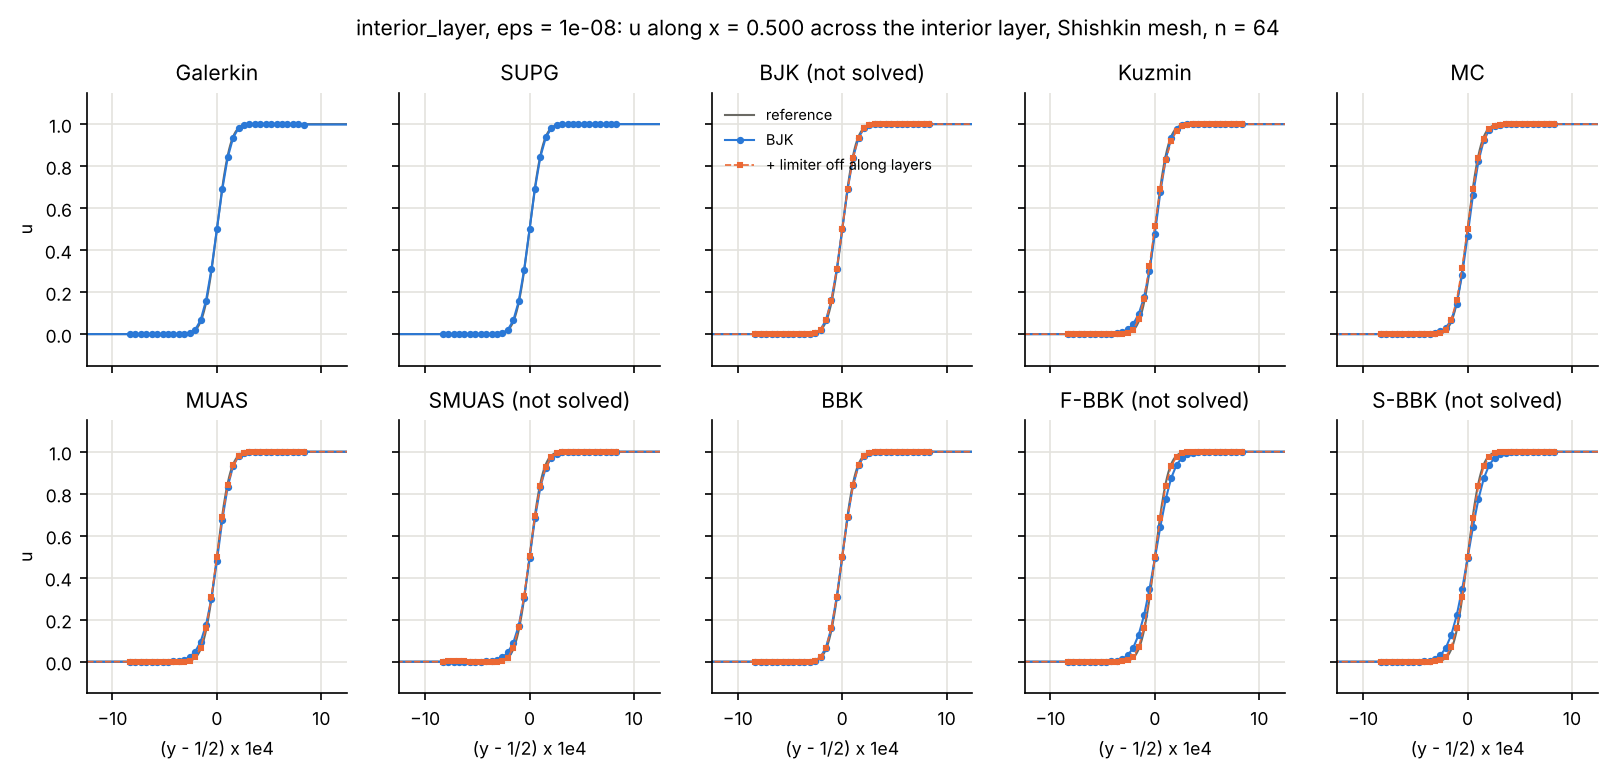
\includegraphics[width=\textwidth]{interior_cut_shishkin_n64.png}
\caption{Example~4: $u_h$ along $x\approx\frac12$ across the interior layer, $|y-\frac12|\le1.5\tau_y$, Shishkin mesh,
$n=64$; grey: reference solution; orange: stabilization switched off along the layers.}\label{fig:interior-cut}
\end{figure}

\begin{figure}[!htbp]\centering
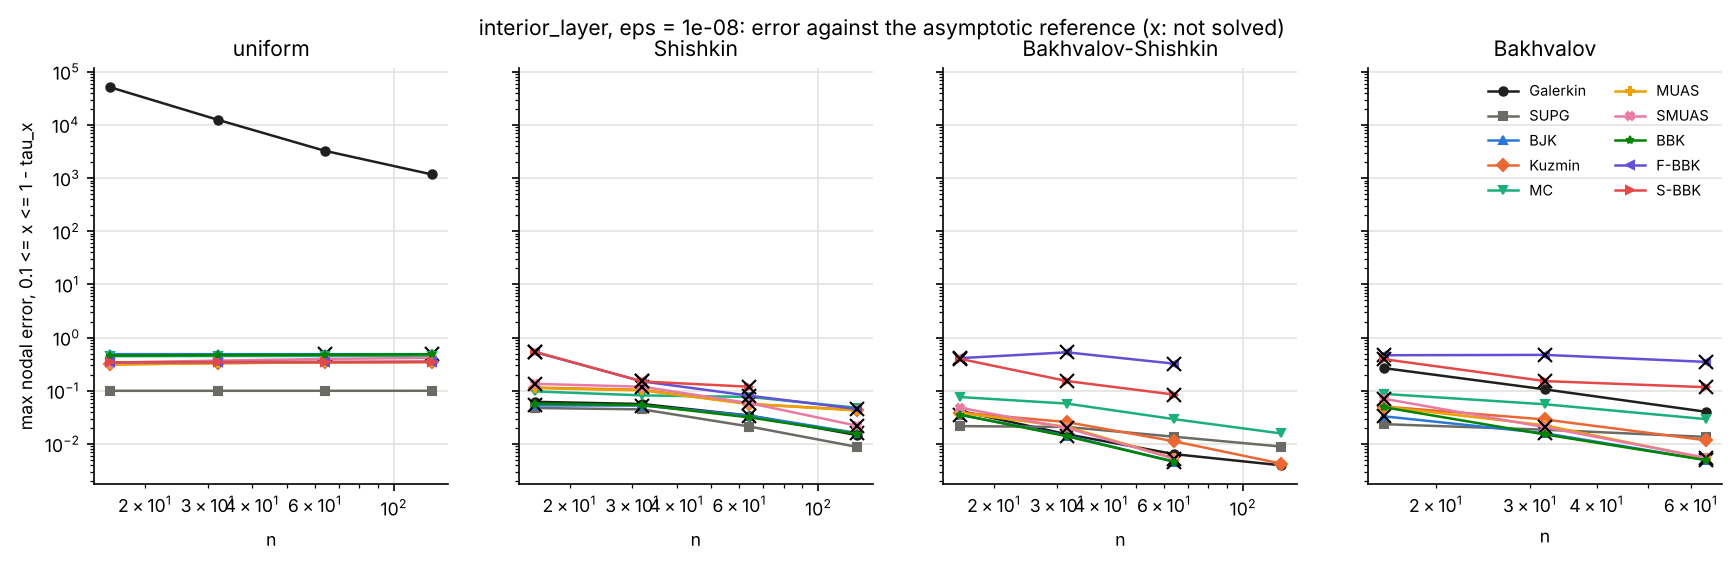
\includegraphics[width=\textwidth]{interior_errors.png}
\caption{Example~4: maximal nodal error for $0.1\le x\le1-\tau_x$; crosses: nonlinear problem not
solved.}\label{fig:interior-err}
\end{figure}

For this problem the algebraic stabilizations are the most accurate methods (Table~\ref{tab:interior},
Figures~\ref{fig:interior-cut} and~\ref{fig:interior-err}). On the Bakhvalov--Shishkin and Bakhvalov meshes, BBK, MUAS
and SMUAS have $L^2$ errors of $3.3$--$4.3\cdot10^{-5}$ at $n=64$, 30 times smaller than the Galerkin method
($1.2\cdot10^{-3}$) and 5 times smaller than the SUPG method ($2\cdot10^{-4}$), and they satisfy $u_h\le1$, whereas the
Galerkin and SUPG methods overshoot by 0.4--1.8\,\%. The solution is monotone across the layer, so that the limiters
have no genuine extremum to clip. The Bakhvalov-type meshes are better than the Shishkin mesh by about a factor of 10
in the errors of all methods; here the abrupt transition of the Shishkin mesh at the edge of the layer region costs
accuracy. Switching the stabilization off along the layers reduces the maximal error of some methods (Kuzmin on the
Bakhvalov--Shishkin mesh: $1.1\cdot10^{-2}\to4.4\cdot10^{-3}$) but leads to overshoots of 0.3--0.6\,\%. On the uniform
mesh the layer is not resolved: the Galerkin solution is useless, and the algebraic stabilizations smear the layer
over a width about 100 times the reference width.

\subsection{Layers along circular arcs}

In Example~5 we compare four meshes with about $n\times n$ cells: the uniform mesh, the polar mesh, the layer-adapted
polar mesh with refinement across $r=0.375$ and $r=0.625$ ($n/4$ rings each) and $r=0.5$, $r=0.75$ ($n/10$ rings
each), half-width $2\sqrt\eps\ln n$, and a tensor-product mesh refined in $x$ and $y$ at the same four values. The
last one is anisotropic, but it is aligned with the arcs only near the inflow and outflow boundaries. For the Neumann
vertices, BJK uses the convex hull of the patch to define its parameter $\gamma_i$, and SMUAS uses no reflected
values. We present results for $n\le64$.

% generated by galerkit examples/convection_diffusion/2d/anisotropic_afc/make_report.py; do not edit
\begin{table}[!htbp]
\centering\scriptsize\setlength{\tabcolsep}{3pt}
\caption{\texttt{rotating\_profile}, $\varepsilon=10^{-5}$, $n=64$: $L^2$ error ($r\le1$) against the radial reference and undershoot $-\min u_h$ (the overshoots are below $2\cdot10^{-5}$ except Galerkin/SUPG on the uniform and tensor meshes, $0.02$--$0.3$); + off: limiter switched off along the layers (aspect threshold 3); $\mu=2$: relaxed limiter; $^*$: nonlinear problem not solved.}\label{tab:rotating}
\resizebox{\textwidth}{!}{\begin{tabular}{l rr rr rr rr}
\toprule
 & \multicolumn{2}{c}{uniform} & \multicolumn{2}{c}{polar} & \multicolumn{2}{c}{polar, layer-adapted} & \multicolumn{2}{c}{tensor, layer-refined}\\
method & $L^2$ & under. & $L^2$ & under. & $L^2$ & under. & $L^2$ & under.\\
\midrule
Galerkin & $5.6\mathrm{e}{-2}$ & $1.6\mathrm{e}{-1}$ & $2.1\mathrm{e}{-2}$ & $4.6\mathrm{e}{-2}$ & $1.2\mathrm{e}{-2}$ & $4.5\mathrm{e}{-2}$ & $7.2\mathrm{e}{-2}$ & $4.5\mathrm{e}{-1}$ \\
SUPG & $5.3\mathrm{e}{-2}$ & $7.9\mathrm{e}{-2}$ & $2.2\mathrm{e}{-2}$ & $2.2\mathrm{e}{-2}$ & $1.3\mathrm{e}{-2}$ & $2.4\mathrm{e}{-2}$ & $6.3\mathrm{e}{-2}$ & $1.1\mathrm{e}{-1}$ \\
BJK & $5.9\mathrm{e}{-2}$ & 0 & $4.1\mathrm{e}{-2}$$^*$ & $3.9\mathrm{e}{-6}$ & $4.2\mathrm{e}{-2}$$^*$ & 0 & $6.5\mathrm{e}{-2}$$^*$ & 0 \\
BJK + off & -- & -- & $4.0\mathrm{e}{-2}$$^*$ & $3.2\mathrm{e}{-2}$ & $1.7\mathrm{e}{-2}$$^*$ & $3.4\mathrm{e}{-2}$ & $6.2\mathrm{e}{-2}$$^*$ & $3.3\mathrm{e}{-1}$ \\
BJK, $\mu=2$ & $5.4\mathrm{e}{-2}$$^*$ & 0 & $9.1\mathrm{e}{-2}$$^*$ & $3.7\mathrm{e}{-2}$ & $3.1\mathrm{e}{-2}$$^*$ & $1.8\mathrm{e}{-8}$ & $6.2\mathrm{e}{-2}$$^*$ & $2.4\mathrm{e}{-6}$ \\
Kuzmin & $6.8\mathrm{e}{-2}$ & 0 & $7.1\mathrm{e}{-2}$ & 0 & $6.8\mathrm{e}{-2}$ & 0 & $1.0\mathrm{e}{-1}$ & 0 \\
Kuzmin + off & -- & -- & $7.0\mathrm{e}{-2}$ & $6.8\mathrm{e}{-3}$ & $5.1\mathrm{e}{-2}$ & $7.5\mathrm{e}{-3}$ & $8.4\mathrm{e}{-2}$ & $3.0\mathrm{e}{-1}$ \\
Kuzmin, $\mu=2$ & $6.1\mathrm{e}{-2}$ & 0 & $5.4\mathrm{e}{-2}$$^*$ & $3.0\mathrm{e}{-6}$ & $5.7\mathrm{e}{-2}$ & 0 & $8.3\mathrm{e}{-2}$ & 0 \\
MC & $6.6\mathrm{e}{-2}$ & 0 & $6.8\mathrm{e}{-2}$ & 0 & $6.3\mathrm{e}{-2}$ & 0 & $9.3\mathrm{e}{-2}$ & 0 \\
MC + off & -- & -- & $6.7\mathrm{e}{-2}$ & $3.2\mathrm{e}{-3}$ & $2.9\mathrm{e}{-2}$ & $4.3\mathrm{e}{-3}$ & $7.7\mathrm{e}{-2}$ & $3.5\mathrm{e}{-1}$ \\
MUAS & $6.8\mathrm{e}{-2}$ & 0 & $7.1\mathrm{e}{-2}$ & 0 & $6.8\mathrm{e}{-2}$ & 0 & $1.0\mathrm{e}{-1}$ & 0 \\
MUAS + off & -- & -- & $6.9\mathrm{e}{-2}$ & $3.5\mathrm{e}{-3}$ & $2.9\mathrm{e}{-2}$ & $2.9\mathrm{e}{-3}$ & $8.2\mathrm{e}{-2}$ & $3.4\mathrm{e}{-1}$ \\
MUAS, $\mu=2$ & $6.1\mathrm{e}{-2}$ & 0 & $5.4\mathrm{e}{-2}$$^*$ & $4.7\mathrm{e}{-6}$ & $5.7\mathrm{e}{-2}$ & 0 & $8.2\mathrm{e}{-2}$ & 0 \\
SMUAS & $8.1\mathrm{e}{-2}$ & 0 & $8.8\mathrm{e}{-2}$ & 0 & $7.3\mathrm{e}{-2}$ & 0 & $1.0\mathrm{e}{-1}$ & 0 \\
SMUAS + off & -- & -- & $8.6\mathrm{e}{-2}$ & $7.0\mathrm{e}{-3}$ & $4.3\mathrm{e}{-2}$ & $7.8\mathrm{e}{-3}$ & $8.8\mathrm{e}{-2}$ & $3.0\mathrm{e}{-1}$ \\
SMUAS, $\mu=2$ & $6.7\mathrm{e}{-2}$ & 0 & $6.7\mathrm{e}{-2}$ & 0 & $6.2\mathrm{e}{-2}$ & 0 & $8.3\mathrm{e}{-2}$ & 0 \\
BBK & $5.9\mathrm{e}{-2}$ & 0 & $4.6\mathrm{e}{-2}$$^*$ & $4.8\mathrm{e}{-6}$ & $5.1\mathrm{e}{-2}$ & 0 & $7.3\mathrm{e}{-2}$ & 0 \\
BBK + off & -- & -- & $4.5\mathrm{e}{-2}$ & $2.6\mathrm{e}{-2}$ & $1.9\mathrm{e}{-2}$ & $2.6\mathrm{e}{-2}$ & $6.7\mathrm{e}{-2}$ & $3.0\mathrm{e}{-1}$ \\
F-BBK & $8.1\mathrm{e}{-2}$$^*$ & $8.9\mathrm{e}{-6}$ & $1.3\mathrm{e}{-1}$$^*$ & $3.3\mathrm{e}{-4}$ & $9.4\mathrm{e}{-2}$$^*$ & 0 & $1.2\mathrm{e}{-1}$$^*$ & $3.5\mathrm{e}{-3}$ \\
F-BBK + off & -- & -- & $7.3\mathrm{e}{-2}$$^*$ & $3.5\mathrm{e}{-3}$ & $4.5\mathrm{e}{-2}$$^*$ & $4.6\mathrm{e}{-3}$ & $1.1\mathrm{e}{-1}$$^*$ & $3.3\mathrm{e}{-2}$ \\
S-BBK & $8.1\mathrm{e}{-2}$$^*$ & $8.9\mathrm{e}{-6}$ & $1.3\mathrm{e}{-1}$$^*$ & $2.6\mathrm{e}{-5}$ & $6.8\mathrm{e}{-2}$ & 0 & $1.1\mathrm{e}{-1}$ & $2.7\mathrm{e}{-4}$ \\
S-BBK + off & -- & -- & $7.4\mathrm{e}{-2}$$^*$ & $3.2\mathrm{e}{-3}$ & $5.4\mathrm{e}{-2}$$^*$ & $4.5\mathrm{e}{-3}$ & $9.8\mathrm{e}{-2}$$^*$ & $3.8\mathrm{e}{-2}$ \\
\bottomrule
\end{tabular}}
\end{table}


\begin{figure}[!htbp]\centering
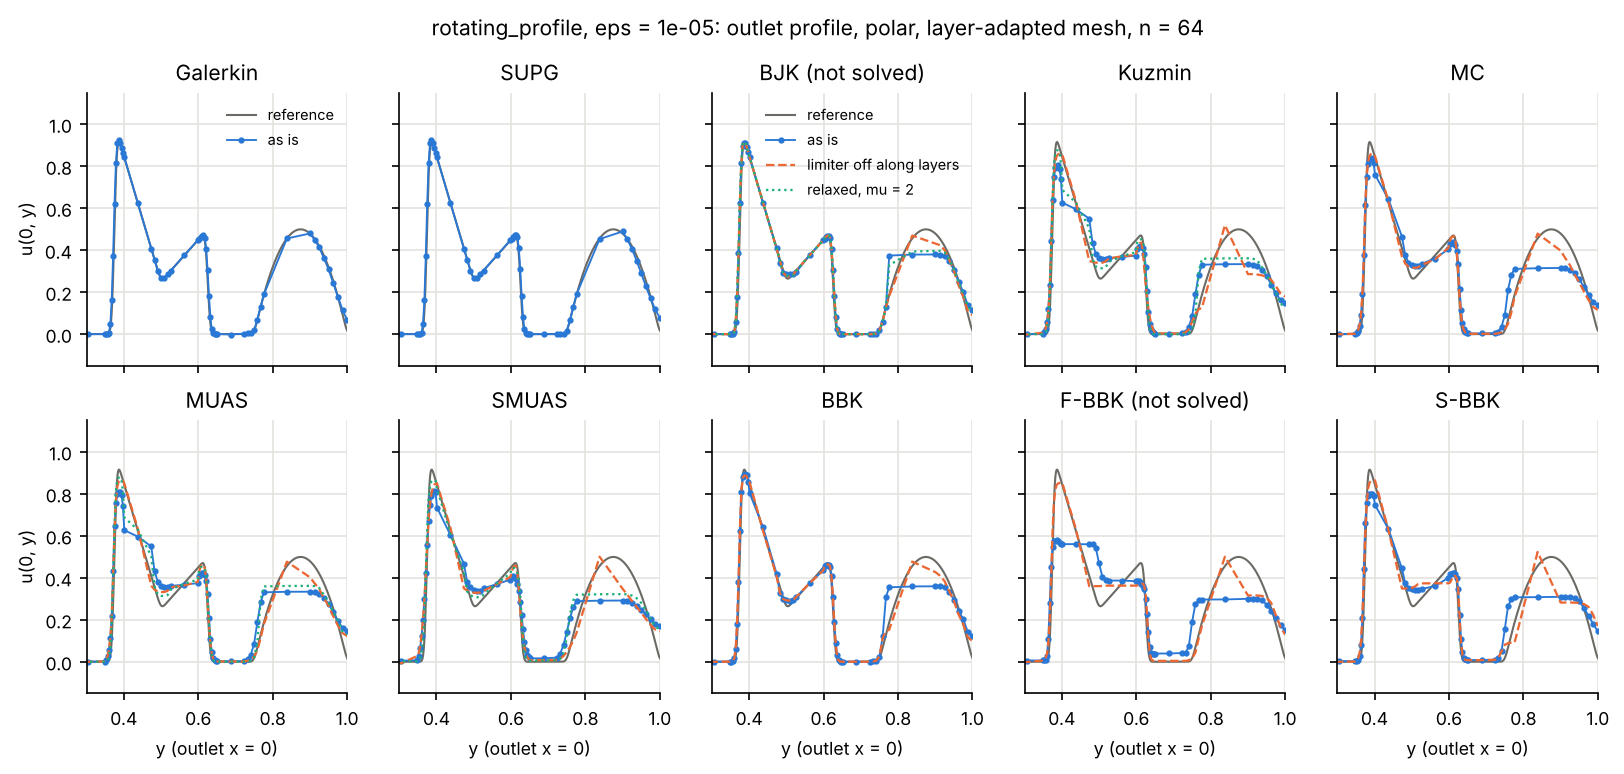
\includegraphics[width=\textwidth]{rotating_outlet_polar_layer_n64.png}
\caption{Example~5: outlet profile $u_h(0,y)$ on the layer-adapted polar mesh, $n=64$; grey: reference solution;
blue: method; orange: stabilization switched off along the layers; green: relaxed limiter $\mu=2$.}\label{fig:rot-outlet}
\end{figure}

\begin{figure}[!htbp]\centering
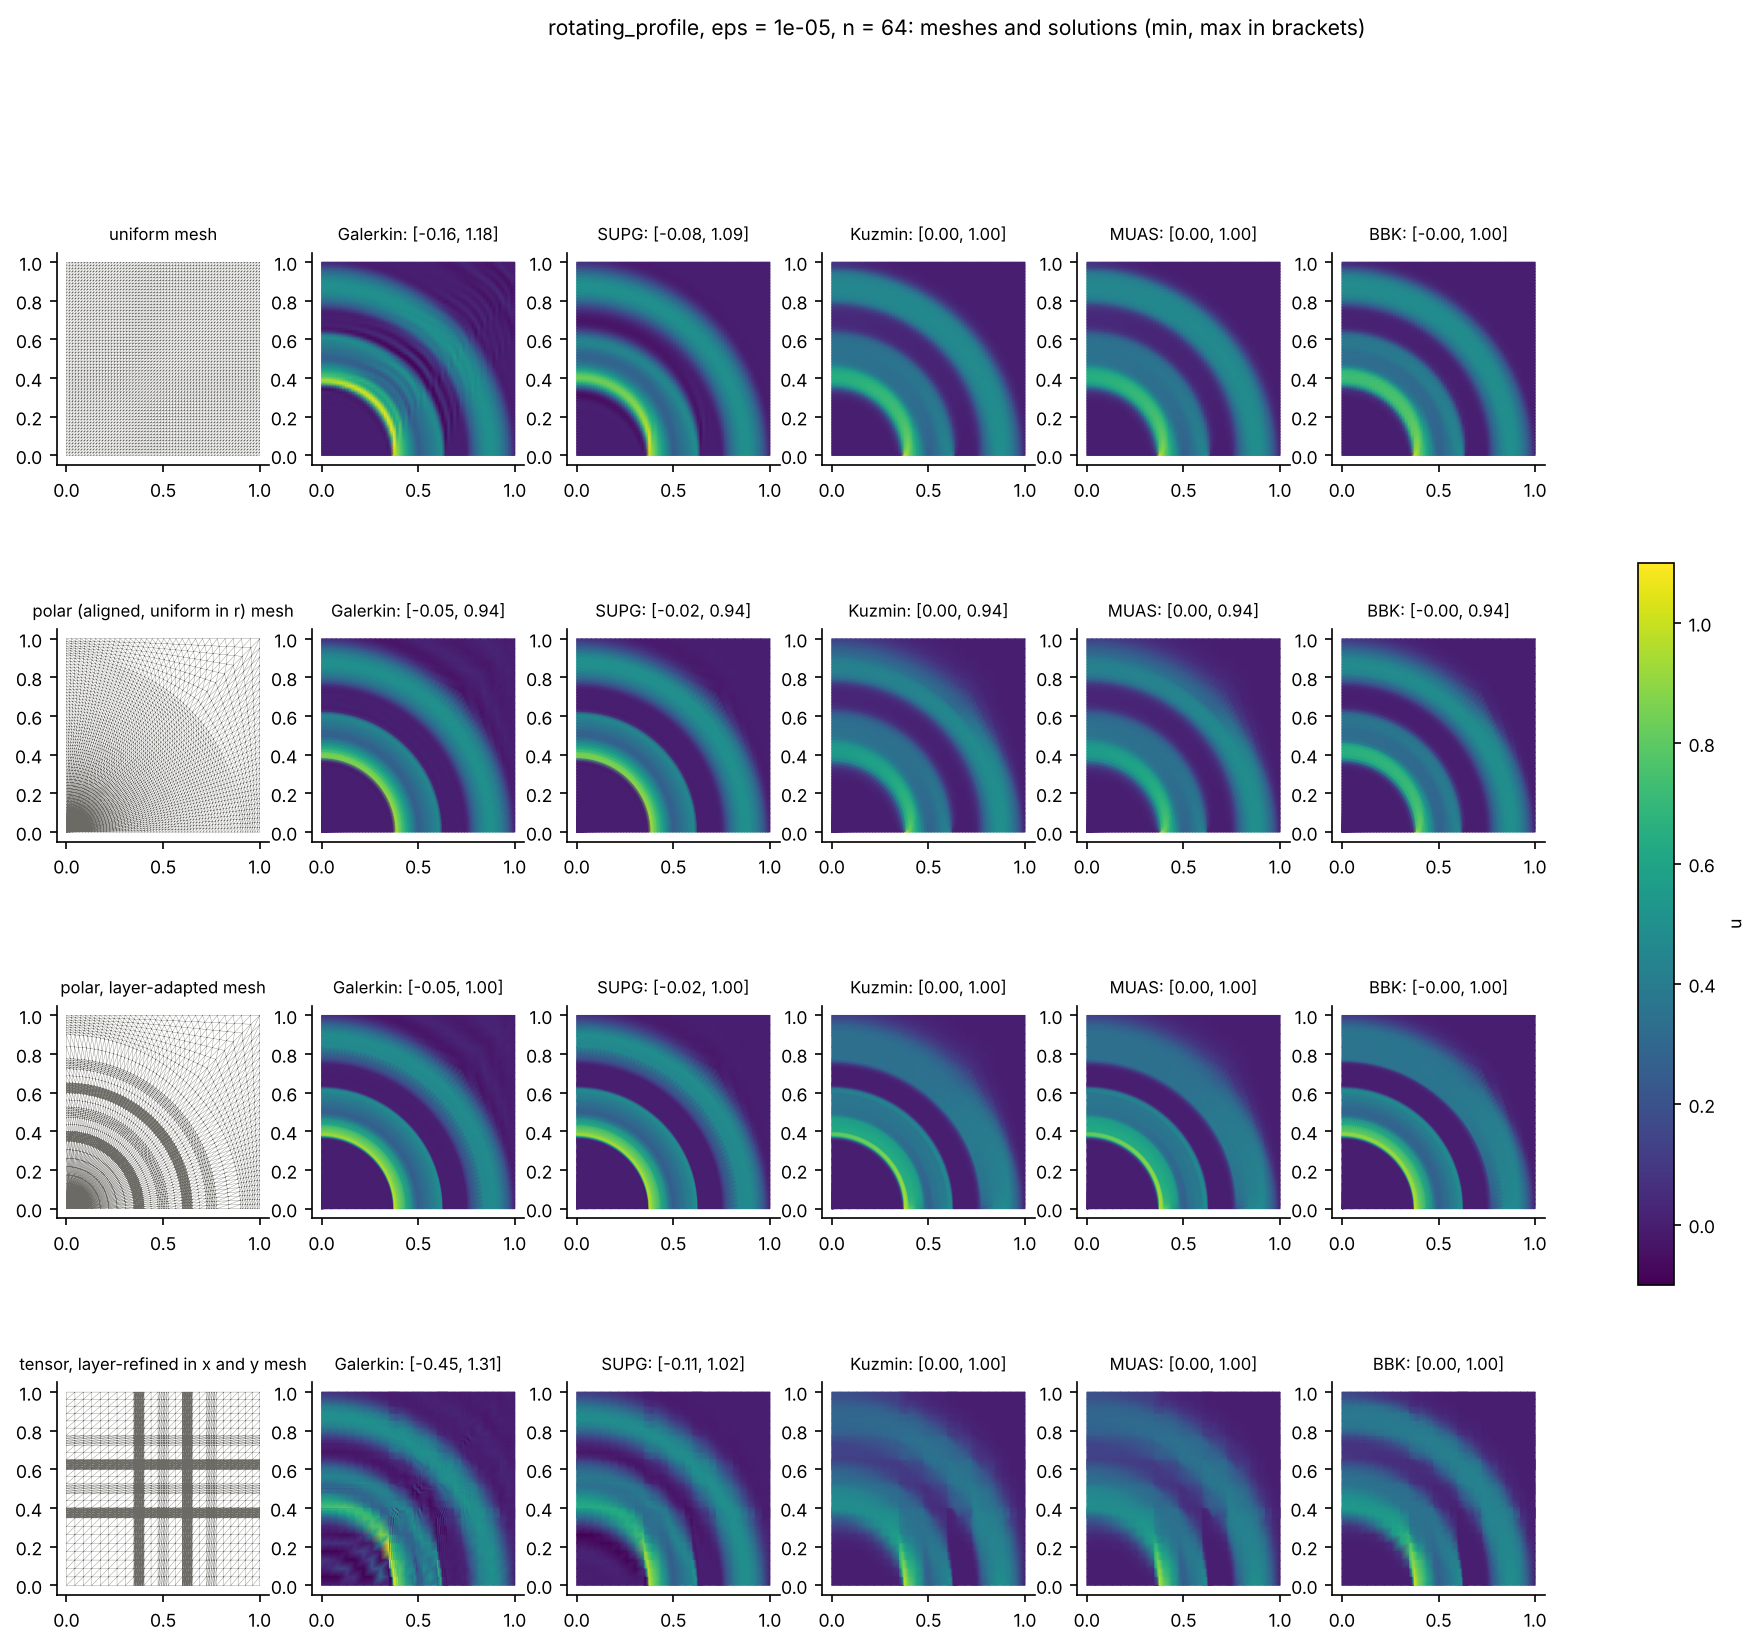
\includegraphics[width=\textwidth]{rotating_solutions_n64.png}
\caption{Example~5, $n=64$: the four meshes and the solutions of the Galerkin, SUPG, Kuzmin, MUAS and BBK methods
($\min u_h$, $\max u_h$ in brackets).}\label{fig:rot-sol}
\end{figure}

Here, the mesh is the decisive factor (Table~\ref{tab:rotating}, Figure~\ref{fig:rot-sol}). The layer-adapted polar
mesh is the best mesh for every method. The tensor-product mesh refined in $x$ and $y$ is the worst for every method,
even worse than the uniform mesh, since in the middle of the domain it is fine in directions that do not cross the
arcs.

On the layer-adapted polar mesh, the Galerkin and SUPG methods are the most accurate ($L^2$ errors
$1.2$--$1.3\cdot10^{-2}$ at $n=64$), but they undershoot by 2--5\,\%. The algebraic stabilizations satisfy
$0\le u_h\le1$ and are 3.5--6 times less accurate. Figure~\ref{fig:rot-outlet} shows the reason: the limiters cannot
distinguish the genuine extrema of the profile, i.e., the peak behind $r=0.375$, the minimum at the kink $r=0.5$, and
the top of the hump, from spurious oscillations. They switch to the low-order scheme at these extrema along the whole
characteristic and clip them; in addition, the diagonal edges of the polar cells contribute crosswind diffusion.
Switching the stabilization off along the layers closes most of the gap on this mesh: BBK reaches $1.9\cdot10^{-2}$,
BJK $1.7\cdot10^{-2}$ (for the best iterate, its nonlinear problem was not solved), and MC and MUAS improve from $6.8\cdot10^{-2}$ to $2.9\cdot10^{-2}$, recovering the peak and most
of the hump. The price is undershoots of 0.3--0.4\,\% for MC and MUAS and 3\,\% for BJK and BBK. On the misaligned
tensor-product mesh, the switch is harmful and leads to undershoots of 30\,\%. The relaxed limiter with $\mu=2$
preserves the bounds but helps little (Kuzmin and MUAS: $6.8\cdot10^{-2}\to5.7\cdot10^{-2}$). The quantities of
interest of \cite{arXiv2204} were not available to us; the measures above are our own.

%=====================================================================================================
\section{Concluding remarks}\label{sec:concl}
%=====================================================================================================

We studied eight algebraically stabilized $P_1$ finite element methods on layer-adapted meshes with aspect ratios up to
$6\cdot10^7$. The main observations are as follows.
\begin{enumerate}[leftmargin=*]
\item All methods resolve exponential and parabolic layers on Shishkin meshes, uniformly in $\eps$. On these meshes,
  however, the Galerkin method is stable, and the algebraic stabilizations are up to 40 times less accurate, with an
  error that concentrates at the transition corner and stems from the diffusion added along the long edges in the
  layer regions.
\item The sufficient conditions for the DMP hold on Shishkin meshes split into right triangles and fail on the
  crossed splitting, without any observed violation of the DMP. Splitting into right triangles is the safe choice.
\item The nonlinear problems become much harder on anisotropic meshes. Switching the stabilization off on the long
  edges along the layers reduces the number of fixed point iterations by factors of 3--50, while the type of the
  layer-adapted mesh changes it by at most a factor of 2. Together with a safeguarded Anderson acceleration, the
  Kuzmin and MUAS methods need 4--6 iterations for an exponential layer and about 35 for layers in two directions.
  Newton's method for regularized limiters with continuation solves BBK where all fixed point variants fail.
\item For a straight interior layer, the algebraic stabilizations on Bakhvalov-type meshes are the most accurate
  methods and satisfy the bounds. For layers along curved arcs, a layer-aligned mesh is essential, and the limiters
  clip the genuine extrema of the solution unless the stabilization is switched off along the layers.
\end{enumerate}
In future work, we plan to study limiters that do not clip smooth extrema, a solution-based criterion for switching
off the stabilization, anisotropic meshes that are not aligned with the coordinate axes, and the three-dimensional
case. The remaining failures of the nonlinear solvers for BJK, SMUAS, F-BBK and S-BBK call for a better
understanding of the solvability and uniqueness of the corresponding nonlinear problems.

%=====================================================================================================
\begin{thebibliography}{99}
% TODO: verify all bibliographic data (entries marked "check").

\bibitem{ABR17} A. Allendes, G.R. Barrenechea, R. Rankin, Fully computable error estimation of a nonlinear,
positivity-preserving discretization of the convection--diffusion--reaction equation, SIAM J. Sci. Comput. 39 (2017)
A1903--A1927. % check

\bibitem{AJ27} N. Ahmed, A. Jha, J. Comput. Phys. 568 (2027). % check: title, authors, pages

\bibitem{arXiv2204} % TODO: authors and title
arXiv:2204.07480, Section~7.

\bibitem{BB17} S. Badia, J. Bonilla, Monotonicity-preserving finite element schemes based on differentiable nonlinear
stabilization, Comput. Methods Appl. Mech. Engrg. 313 (2017) 133--158. % check

\bibitem{Bak69} N.S. Bakhvalov, The optimization of methods of solving boundary value problems with a boundary layer,
USSR Comput. Math. Math. Phys. 9 (1969) 139--166. % check

\bibitem{BBK17} G.R. Barrenechea, E. Burman, F. Karakatsani, Edge-based nonlinear diffusion for finite element
approximations of convection--diffusion equations and its relation to algebraic flux-correction schemes, Numer. Math.
135 (2017) 521--545.

\bibitem{BJK16} G.R. Barrenechea, V. John, P. Knobloch, Analysis of algebraic flux correction schemes, SIAM J. Numer.
Anal. 54 (2016) 2427--2451.

\bibitem{BJK17} G.R. Barrenechea, V. John, P. Knobloch, An algebraic flux correction scheme satisfying the discrete
maximum principle and linearity preservation on general meshes, Math. Models Methods Appl. Sci. 27 (2017) 525--548.

\bibitem{BH82} A.N. Brooks, T.J.R. Hughes, Streamline upwind/Petrov--Galerkin formulations for convection dominated
flows with particular emphasis on the incompressible Navier--Stokes equations, Comput. Methods Appl. Mech. Engrg. 32
(1982) 199--259.

\bibitem{DL06} R.G. Dur\'an, A.L. Lombardi, Finite element approximation of convection diffusion problems using
graded meshes, Appl. Numer. Math. 56 (2006) 1314--1325. % check

\bibitem{JJ19} A. Jha, V. John, A study of solvers for nonlinear AFC discretizations of convection--diffusion equations,
Comput. Math. Appl. 78 (2019) 3117--3138. % check

\bibitem{JK07} V. John, P. Knobloch, On spurious oscillations at layers diminishing (SOLD) methods for
convection--diffusion equations: Part I -- A review, Comput. Methods Appl. Mech. Engrg. 196 (2007) 2197--2215.

\bibitem{JK22} V. John, P. Knobloch, On algebraically stabilized schemes for convection--diffusion--reaction problems,
Numer. Math. 152 (2022) 553--585. % check

\bibitem{Kno23} P. Knobloch, An algebraically stabilized method for convection--diffusion--reaction problems with
optimal experimental convergence rates on general meshes, Numer. Algorithms 94 (2023) 547--580. % check

\bibitem{Kuz07} D. Kuzmin, Algebraic flux correction for finite element discretizations of coupled systems, in:
Computational Methods for Coupled Problems in Science and Engineering II, CIMNE, Barcelona, 2007, 653--656. % check

\bibitem{Kuz20} D. Kuzmin, Monolithic convex limiting for continuous finite element discretizations of hyperbolic
conservation laws, Comput. Methods Appl. Mech. Engrg. 361 (2020) 112804.

\bibitem{Lin10} T. Lin{\ss}, Layer-Adapted Meshes for Reaction-Convection-Diffusion Problems, Lecture Notes in
Mathematics 1985, Springer, Berlin, 2010.

\bibitem{MOS96} J.J.H. Miller, E. O'Riordan, G.I. Shishkin, Fitted Numerical Methods for Singular Perturbation
Problems, World Scientific, Singapore, 1996.

\bibitem{RST08} H.-G. Roos, M. Stynes, L. Tobiska, Robust Numerical Methods for Singularly Perturbed Differential
Equations, 2nd ed., Springer, Berlin, 2008.

\bibitem{WN11} H.F. Walker, P. Ni, Anderson acceleration for fixed-point iterations, SIAM J. Numer. Anal. 49 (2011)
1715--1735.

\end{thebibliography}

\end{document}
